\section{Estructura general}

    El laboratorio virtual de sistemas de control clásicos y difusos fue pensado de modo que cada una de sus funcionalidades principales sean independientes la una de la otra, no obstante, ciertas rutinas son comunes entre ellas. Por otro lado, se organizo la aplicación de modo que cada funcionalidad principal posea un archivo \enquote{handler}, el cual hará de intermediario entre la interfaz gráfica y las rutinas de calculo que se encuentran en un archivo de rutinas. La \cref{fig:estructuraMain} sirve como referencia de la estructura general utilizada.

    \begin{figure}[htb]
        \centering
        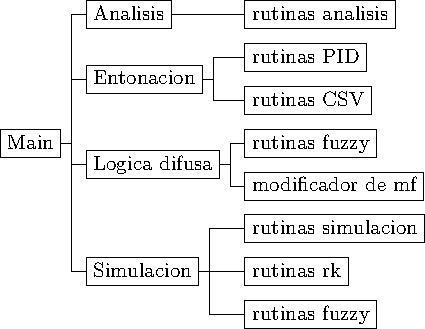
\includegraphics[width=0.8\textwidth]{estructuraMain.pdf}
        \caption[Diagrama general de la aplicación]{\textbf{Diagrama general de la aplicación}. La estructura general de la aplicación, la segunda columna representa a los archivos handler mientras que la tercera son los archivos de rutinas. Fuente: Elaboración propia.} 
        \label{fig:estructuraMain}
    \end{figure}

\section{Análisis de sistemas de control}
    
    Con esta función se quiso dar la posibilidad de realizar los análisis en el tiempo y en frecuencia típicos para un proceso ingresado por el usuario, los análisis típicos son: respuesta al escalón, respuesta al impulso, diagrama de bode, diagrama de Nyquist, lugar de las raíces y diagrama de Nichols. El \cref{code:analisis} muestra un pseudo código de la funcionalidad de análisis de sistemas de control y la interfaz grafica correspondiente se puede observar en el \ref{anexo:interfazAnalisis}.

    \begin{longlisting}
        \caption[Pseudo código - Análisis de sistemas de control]{Pseudo código para el análisis de sistemas de control}
        \label{code:analisis}				
        \begin{minted}[escapeinside=||,
            mathescape=true,
            autogobble=true,
            fontsize=\footnotesize,
            obeytabs=true,
            tabsize=4,
            baselinestretch=1]{text}
            |\bf{WHILE}| True: # Ciclo principal
                |$\vdots$|
                |\bf{IF}| validaciones_entradas_análisis:
                    validar_entrada_análisis()
                
                |\bf{IF}| usuario_presiona_calcular:
                    chequeo_TF_SS()
                    creación_proceso()
                    escalón()
                    impulso()
                    bode()
                    nyquist()
                    lugar_de_las_raíces()
                    nichols()
                    datos()
                |$\vdots$|
        \end{minted}
    \end{longlisting}

    Inicialmente se valida cada una de las entradas del usuario y se chequea si el botón para realizar los cálculos fue presionado. Una vez presionado el botón de calcular se procede a verificar la representación del sistema y a crearlo para a continuación ejecutar las rutinas de análisis.

    \subsection{Definición del proceso}

        Un proceso deberá ser ingresado para poder realizar el análisis, la entonación o la simulación del mismo. El sistema puede ser definido con los coeficientes del numerador y el denominador de la función de transferencia o puede ser definido ingresando las matrices A, B, C y D de la ecuación de espacio de estados. En ambos casos se deben cumplir con los principios matemáticos que correspondan, i.g., las función de transferencia no puede ser impropia.

    \subsubsection{Tiempo discreto}

        La opción de discretizacion permite llevar el proceso ingresado en tiempo continuo a una aproximación en tiempo discreto con solo ingresar el periodo de muestreo y seleccionar el método a utilizar. Se implementaron los siguientes métodos de discretizacion:

        \begin{enumerate}[leftmargin=\parindent]
            \item Retensor de orden cero  (ZOH)
            \item Retensor de primer orden (FOH)
            \item Euler hacia atrás (backward\_diff)
            \item Euler hacia adelante (Euler)
            \item Transformación bilineal (Tustin)
            \item Transformación directa de polos y ceros (matched)
            \item Transformación del impulso invariante (impulse)
        \end{enumerate}

    \subsubsection{Proceso con atraso o delay}
        
        A los procesos ingresados se les puede agregar un atraso, este atraso es manejado de forma distinta dependiendo de la funcionalidad. Para el caso de la funcionalidad de análisis, el delay fue implementado para la respuesta escalón y la respuesta impulso como un desplazamiento en el tiempo equivalente al delay ingresado, para la respuesta en frecuencia se multiplico $e^{-j\omega \alpha}$ a cada una de las evaluaciones de frecuencia con $\alpha$ como el delay ingresado por el usuario. Para el caso del lugar de las raíces, el delay es implementado utilizando una aproximación por PADE.

        Si el proceso es definido en tiempo discreto el mismo es multiplicado por $z^{-\alpha/T}$ con la idea de retrasar las muestras en un numero equivalente al delay deseado, de este modo, no hay casos especiales dependiendo del tipo de análisis.

    \subsection{Respuesta al escalón}
        
        Se obtiene la respuesta en el tiempo del sistema en lazo abierto ante una entrada escalón de amplitud uno, con los datos de la respuesta se realiza la gráfica correspondiente.
    
    \subsection{Respuesta al impulso}
        
        Se obtiene la respuesta en el tiempo del sistema en lazo abierto ante un impulso como entrad al sistema, con los datos de la respuesta se realiza la gráfica correspondiente.

    \subsection{Diagrama de Bode}
        
        Se obtiene la respuesta en frecuencia del sistema, con los datos de la respuesta en frecuencia se realiza las gráficas de magnitud y fase. Adicional a las gráficas fue implementado el calculo de los margenes de ganancia y de fase, la implementación fue realizada desde cero debido a los resultados inaceptables obtenidos con la implementación de la librería de control. El código para el calculo de los margenes de ganancia y fase se puede observar en el \ref{anexo:margenes}.
    
    \subsection{Diagrama de Nyquist}
        
        El diagrama de Nyquist también fue realizado utilizando la librería de control, en el mismo se señala la dirección de la gráfica y el punto $-1 + j0$. Las frecuencias utilizadas son las mismas utilizadas para el diagrama de Bode dado que las mismas son calculadas de manera automática por la librería de control en ambos casos.
    
    \subsection{Gráfica del lugar de las raíces}
        
        La gráfica es realizada utilizando la librería de control, una de las funciones que posee es poder seleccionar cualquier punto en la gráfica y obtener la ganancia y el damping que le corresponden. Para el caso de sistemas discretos se grafica el circulo unitario.
    
    \subsection{Diagrama de Nichols}
        
        A diferencia del diagrama de Nyquist aca se señala el punto $(0dB, -180^\circ)$, la librería de controla ya viene con la opción para superponer una rejilla que representa a la Carta de Nichols.

    \subsection{Despliegue de datos}
        
        Los datos obtenidos se muestran de forma escrita, los datos a desplegar son: el sistema ingresado, los datos de la respuesta al escalón, los margenes de ganancia y fase, los valores eigen y su respectivo damping.

\section{Entonación de controladores PID}

    Esta función fue dividida en dos apartados, el primero, es la entonación de un proceso en lazo cerrado con un controlador PID,las ganancias del controlador son ajustables por el usuario, adicionalmente, se puede realizar una entonación automática utilizando el método de Ziegler-Nichols o Cohen-Coon. La segunda opción permite cargar la data de respuesta ante un escalón desde un archivo CSV para realizar la entonación. El \cref{code:entonacion} muestra un pseudo código de la funcionalidad de entonación de controladores PID y la interfaz grafica correspondiente se puede observar en el \ref{anexo:interfazentonacion}.
    
    \begin{longlisting}
        \caption[Pseudo código - Entonación de controladores PID]{Pseudo código para la entonación de controladores PID}
        \label{code:entonacion}				
        \begin{minted}[escapeinside=||,
            mathescape=true,
            autogobble=true,
            fontsize=\footnotesize,
            obeytabs=true,
            tabsize=4,
            baselinestretch=1]{text}
            |\bf{WHILE}| True: # Ciclo principal
                |$\vdots$|
                |\bf{IF}| validaciones_entradas_entonación:
                    validar_entrada_entonación()
                |\bf{IF}| usuario_presiona_calcular:
                    |\bf{CASO 1}| entonación_manual:
                        chequeo_TF_SS()
                        creación_proceso()
                        entonación()
                        escalón()
                    |\bf{CASO 2}| entonación_automática:
                        chequeo_TF_SS()
                        creación_proceso()
                        escalón()
                    |\bf{CASO 3}| entonación_CSV:
                        procesar_CSV()
                        entonación()
                        graficacion()
                |$\vdots$|
        \end{minted}
    \end{longlisting}

    El forma de definición de procesos presentado en la funcionalidad de análisis de sistemas de control es reutilizada para esta sección. Al igual que para el análisis de sistemas de control, inicialmente se valida cada una de las entradas del usuario y se chequea si el botón para realizar los cálculos fue presionado, una vez presionado el botón de calcular se procede a verificar que tipo de calculo se va a realizar entre: entonación manual, entonación automática o entonación con archivo CSV.

    \subsection{Entonación de sistema en lazo cerrado con PID}
        
        Para el calculo de la respuesta al escalón se utiliza la librería de control, el esquema implementado es el presentado en la \cref{fig:esquemaPID}. El controlador PID fue definido utilizando \cref{eq:pidcompleja} y sustituyendo la componente derivativa por \cref{eq:Daproximacion}. Si el sistema es representado en tiempo discreto se utiliza \cref{eq:pidenZ} para definir al controlador PID.
        
        Asi mismo, para la entonación automática se realiza una prueba escalón en lazo abierto con el propósito de calcular \cref{eq:parametroK}, \cref{eq:parametroTau} y \cref{eq:parametroAlfa}, luego, se sustituyen los valores en la \cref{tab:ZiglerNichols,tab:CohenCoon} con el fin de realizar una entonación por el método Ziegler-Nichols y Cohen-Coon según la selección del usuario.

    \subsection{Entonación utilizando un archivo CSV}

        Como ya se menciono, con esta opción se permite cargar un archivo CSV que contenga la data de respuesta a un escalon con la finalidad de obtener su aproximacion de primer orden con tiempo muerto y poder realizar una entonacion utilizando el método de Zigler-Nichols o Cohen-Coon. El usuario debe ingresar el limite superior e inferior de la variable del proceso (Vp) y de la entrada al sistema, normalmente, la señal del elemento final de control (EFC), adiocionalmente, debe ingresar el separador del archivo CSV cuyo valor por defecto es una coma (,).

        El algoritmo aproximara los parámetros de un modelo de primer orden con tiempo muerto utilizando el punto de máxima pendiente para trazar una recta, este punto quedara como ancla permitiendo al usuario ajustar el tiempo $t_1$ en caso de que el ajuste automático no genere buenos resultados. El algoritmo solo funciona para respuestas ascendentes, i.g., como la observada en la \cref{fig:ZNtest}.

        El archivo CSV deberá contener un formato de encabezados especifico, los encabezados deben contener las palabras clave VP, EFC o TIME para identificar las columnas. El algoritmo intentara buscar las palabras clave dentro del encabezado de cada columna, i.g., datavpsimulacion identificaría a los datos de Vp debido a que incluye la palabra clave Vp, no se hace distinción entre minúsculas y mayúsculas. La columna que contiene los datos de tiempo puede expresar el tiempo en los formatos hh:mm:ss, mm:ss o directamente en segundos. Un ejemplo del formato de un CSV valido se puede observar en el \ref{anexo:csv}.

\section{Diseño de controladores difusos}
    
    Para el diseño de controladores difusos se utiliza de fondo la librería Scikit-Fuzzy, la cual permite por medio de código Python diseñar controladores difusos tipo Mamdani, graficar las funciones de membresía y realizar el proceso de inferencia para el controlador diseñado. La mayoría de la funcionalidad consiste en ser un intermediario entre las entradas del usuario por medio de la interfaz gráfica y el código que requiere Scikit-Fuzzy para poder definir un controlador. Adicional a lo anterior, se implemento la posibilidad de cargar y exportar archivos FIS con ciertas limitaciones tanto en la importación como en la exportación. El \cref{code:fuzzylogic} muestra un pseudo código de la funcionalidad de diseño de controladores difusos y la interfaz gráfica correspondiente se puede observar en el \ref{anexo:interfazFuzzy}.

    \begin{longlisting}
        \caption[Pseudo código - Diseño de controladores difusos]{Pseudo código para el diseño de controladores difusos}
        \label{code:fuzzylogic}				
        \begin{minted}[escapeinside=||,
            mathescape=true,
            autogobble=true,
            fontsize=\footnotesize,
            obeytabs=true,
            tabsize=4,
            baselinestretch=1]{text}
            |\bf{WHILE}| True: # Ciclo principal
                |$\vdots$|
                |\bf{IF}| validaciones_entradas_fuzzy:
                    validar_entrada_fuzzy()
                
                |\bf{IF}| usuario_presiona_generar:
                    |\bf{IF}| esquemas == True:
                        empezar_diseño_esquema()
                    |\bf{ELSE}|
                        empezar_diseño_genérico()
                
                |\bf{IF}| usuario_presiona_crear:
                    crear_controlador()
                    prueba_entradas()
                    |\bf{IF}| entradas == 1 |\bf{OR}| entradas == 2:
                        superficie_respuesta()
                |$\vdots$|
        \end{minted}
    \end{longlisting}
    
    \subsection{Controladores difusos}

        Los controladores difusos fueron divididos para su diseño en dos categorías, genéricos y basados en un esquema de control especifico.
        
        \subsubsection{Controladores genericos}

            Los controladores genéricos pueden tener un numero arbitrario de entradas y salidas con un máximo de diez entradas o salidas, al ser genéricos, no se garantiza que puedan ser utilizados en la funcionalidad de simulación de sistemas de control, por tanto, sirve para diseñar cualquier sistema de inferencia difuso con o sin el propósito de utilizarle como controlador.

            \paragraph{Funciones de membresia}

                Scikit-Fuzzy posee todas las funciones de membresías descritas por las ecuaciónes \cref{eq:trimf} a la \cref{eq:gbellmf} junto con las funciones compuestas: gauss2mf, dsigmf, psigmf y pimf. Para poder cambiar entre funciones de membresía se codificaron transformaciones aproximadamente equivalente entre las definiciones de las mismas, se llamo definición a los valores necesarios para poder definir la función de membresía. El código para realizar las transformaciones se puede observar en el \ref{anexo:mfequivalencia}.

            \paragraph{Defuzzificacion}

                Todos los métodos de defuzzificacion descritos en \cref{secc:defuzzificacion} son utilizables con Scikit-Fuzzy y pueden ser asignados de forma individual a cada salida del controlador difuso, i.e., cada salida puede utilizar un método de defuzzificacion distinto.

            \paragraph{Reglas de inferencia}

                Las reglas pueden plantearse utilizando conjunción de premisas o disyunción de premisas, i.e., lógica AND o lógica OR, a su vez, cada una de las premisas pueden ser negadas. A las salidas se les puede asignar un peso de forma individual, de modo que cada salida puede ser ponderada de forma distinta, las salidas no pueden ser negadas.

        \subsubsection{Controladores basados en esquemas}

            Los controladores basados en esquemas poseen todas las características de los controladores difusos a excepción de la posibilidad de seleccionar el numero de entradas, el numero de salidas y los nombres de las variables de entrada y salida, el motivo es que estos controladores están asociados a un esquema de control especifico que debe cumplir con un numero de entradas y salidas ya establecido. Los esquemas de control difuso que se pueden diseñar son los presentados en las \cref{fig:pdFuzzyTomo,fig:piFuzzyTomo,fig:pidFuzzyTomo,fig:GainschedulerTomo,fig:pidplusFuzzyTomo} con ciertos cambios que se detallaran, junto con algunos esquemas extras, en la sección correspondiente a la funcionalidad de simulación. Todos los esquemas de control difuso se pueden observar en el \ref{anexo:esquemas}.

    \subsection{Guardado de controladores difusos}

        \subsubsection{Archivos JSON}
        
            Para guardar el diseño del usuario se utiliza un archivo .JSON con una estructura interna particular y única para funcionar de forma especifica con el laboratorio virtual de sistemas de control, los archivos JSON guardan datos que luego pueden ser cargados de forma directa con la librería JSON de Python. Un ejemplo del formato interno del archivo .JSON para un controlador con una entrada y una salida se puede observar en el \ref{anexo:json}.

        \subsubsection{Archivos FIS}

            Los archivos FIS son otra forma de cargar el controlador difuso o exportarlo, existen ciertas limitaciones en la carga y en el exportado de archivos FIS producto de las posibilidades que ofrece Scikit-Fuzzy.

            \paragraph{Cargar controlador}
            
                 Para la carga del controlador se utiliza una versión modificada del parsin de archivos FIS de YAPFLM (Yet Another Python Fuzzy Logic Module) de \textcite{sputnick1124} para extraer los datos del archivo FIS, luego, otro código es utilizado para llevar los datos extraídos a la estructura presentada en los archivos .JSON. Debido a que Scikit-Fuzzy no permite salidas negadas en las reglas se genera un error en caso de que alguna de las salidas en las reglas se encuentre negada.
            
            \paragraph{Exportar controlador}

                Para realizar el exportado del controlador difuso se realiza un parsin entre la estructura presentado en los archivos .JSON y la de un archivo FIS. En caso de que alguna regla posea pesos diferentes para cada salida solo se tomara en cuenta el peso asociado a la primera salida, esto es debido a que los archivos FIS no permiten pesos individuales por cada salida, lo mismo aplica al método de defuzzificacion, se toma el asignado a la primera salida. El código para realizar la carga y el exportado de archivos FIS se puede observar en el \ref{anexo:codefis}.

\section{Simulación de sistemas de control}

    Esta funcionalidad permite simular sistemas de control en lazo cerrado con un controlador PID clásico, difuso o ambos, adicional al controlador se permite agregar bloques adicionales como accionador, saturador del accionador y/o sensor. Para la simulación se utilizan un método de Runge-Kutta como solucionador y obtener la respuesta en el tiempo del sistema, los esquemas simulables están predefinidos. El \cref{code:simulacion} muestra un pseudo código de la funcionalidad de simulación de sistemas de control y la interfaz gráfica correspondiente se puede observar en el \ref{anexo:interfazSimulacion}.

    \begin{longlisting}
        \caption[Pseudo código - Simulación de sistemas de control]{Pseudo código para la simulación de sistemas de control}
        \label{code:simulacion}				
        \begin{minted}[escapeinside=||,
            mathescape=true,
            autogobble=true,
            fontsize=\footnotesize,
            obeytabs=true,
            tabsize=4,
            baselinestretch=1]{text}
            |\bf{WHILE}| True: # Ciclo principal
                |$\vdots$|
                |\bf{IF}| validaciones_entradas_simulación:
                    validar_entrada_simulación()
                
                |\bf{IF}| usuario_presiona_calcular:
                    chequeo_esquema()
                    datos = recolección_datos()
                    hilo_de_simulación(datos)
                |$\vdots$|
            
            |\bf{FUNCION}| hilo_de_simulación(datos):
                procesar_datos(datos)
                resultados = simular_esquema(método_rk)
                return resultados
        \end{minted}
    \end{longlisting}

    Al igual que para la funcionalidad de análisis de sistemas de control y entonación de controladores PID se reutiliza la forma de ingresar el proceso, por lo que también se realiza la validación de entradas y se monitorea si el usuario presiona el botón de calcular, cuando el usuario presiona calcular, se procede a realizar la simulación del esquema de control seleccionado en un hilo distinto al de la aplicación principal debido a que los tiempos de simulación para los esquemas difusos pueden ser de varios segundos y presentaría un comportamiento de bloqueo para la ventana de la aplicación.

    En caso de que la simulación sea realizada para tiempo discreto, se evaluá \cref{eq:SSdiscreto} en cada iteración para obtener la salida del sistema. Si es el esquema seleccionado es el del PID clásico el controlador implementado es el descrito por \cref{eq:pidcdiscreto}. Si el sistema es continuo, la respuesta del sistema y del controlador es calculada utilizando el método de Runge-Kutta seleccionado.

    \subsection{Esquemas de simulación}

        Para la simulación de sistemas de control se implementaron los esquemas de control presentados en el \cref{sec:esquemasFuzzy} y otros esquemas que se encuentran compuestos de la combinación de los mismos. Como ya se menciono, los esquemas de control se pueden observar en el \ref{anexo:esquemas} y se listan a continuación:

        \begin{enumerate}[leftmargin=\parindent]
            \item PID clásico
            \item PID difuso
            \item PI difuso
            \item PD difuso
            \item PD difuso + PI difuso
            \item PI difuso + Derivada clásica
            \item PD difuso + Integrador clásico
            \item Programador de ganancias
            \item PID clásico + Difuso simple (P)
        \end{enumerate}

        A la derivada de aquellos esquemas que requieran su calculo se les fue agregado una funcion de transferencia en serie con la misma para limitar la respuesta a las altas frecuencias, esto es debido a que las simulaciones se van a realizar con un método de Runge-Kutta que requeriría un tamaño de paso muy pequeño para poder aproximar de forma correcta incluso a una derivada aproximada dada por \cref{eq:Daproximacion}, y un incremento en el numero de pasos provocaría, a su vez, un incremento en los tiempos de simulación para los esquemas con controladores difusos, y en consecuencia, volviendo la herramienta impráctica.

    \subsection{Solución por Runge-Kutta}

        Como ya se menciono, la simulación se llevara acabo utilizando un método de Runge-Kutta, para ello se implementaron múltiples métodos, el usuario puede seleccionar cualquiera de ellos para realizar la simulación. En total se implementaron nueve Runge-Kutta's explícitos y cuatro embebidos. Las tablas de Butcher para cada uno de los métodos implementados se pueden observar en el \ref{anexo:butcher}, a continuación, se presenta una lista de los métodos implementados:

        \begin{enumerate}[leftmargin=\parindent]
            \item Explícitos:
                \begin{enumerate}
                    \item Runge-Kutta de orden 2
                    \item Runge-Kutta de orden 3
                    \item Ralston de orden 3
                    \item Heun de orden 3
                    \item Strong Stability Preserving Runge-Kutta (SSPRK) de orden 3
                    \item Runge-Kutta de orden 4
                    \item Runge-Kutta 3/8 de orden 4
                    \item Ralston con minimo error de truncamiento de orden 4
                    \item Runge-Kutta de orden 5
                \end{enumerate}
            \item Embebidos:
                \begin{enumerate}
                    \item Bogacki-Shampine de orden 3(2)
                    \item Fehlberg  de orden 4(5)
                    \item Cash-Karp de orden 4(5)
                    \item Dormand-Prince de orden 5(4)
                \end{enumerate}
        \end{enumerate}

        Con el fin mejorar la precision y mantener el numero de pasos al minimo se implemento un algoritmo de ajuste del tamaño de paso para los metodos de Runge-Kutta, para el caso de los Runge-Kutta explicitos se implementaron las ecuaciones \cref{eq:escalaDos,eq:ErrorNormalizado,eq:casosStep} y para los embebidos las ecuaciones \cref{eq:escalaEmbebidos,eq:ErrorNormalizado,eq:casosStep}. Los pseudo codigos para los tamaños de paso variable se pueden observar en los \cref{code:stepexplicito,code:stepembebido}, y los codigos en Python se pueden observar en el \ref{anexo:stepsize}.

        El calculo del tamaño de paso se realiza con el bloque que presente mayores variaciones y requiera la mayor presicion, i.e., el menor tamaño de paso, en la mayoria de los casos este bloque es o incluye a la componente derivativa. Para el resto de bloques que requieran ser calculados, se utiliza un Runge-Kutta explicito con tamaño de paso igual al calculado, el Runge-Kutta utilizado varia segun el metodo utilizado.

        \pagebreak

        \begin{longlisting}
            \caption[Pseudo código - Runge-Kutta explicitos]{Pseudo código para el ajuste del tamaño de paso de los Runge-Kutta explicitos.}
            \label{code:stepexplicito}				
            \begin{minted}[escapeinside=||,
                mathescape=true,
                autogobble=true,
                fontsize=\footnotesize,
                obeytabs=true,
                tabsize=4,
                baselinestretch=1]{text}
                |\bf{FUNCION}| Tamaño_de_paso_variable(parametros):
                    |\bf{WHILE}| True:
                        |$y_{h}$|, |$x_{h}$| = calculo_rk(h, |$x$|)
                        _, |$x_{h/2}$| = calculo_rk(h/2, |$x$|)
                        |$y_{h/2}$|, |$x_{h/2}$| = calculo_rk(h/2, |$x_{h/2}$|)
                        escala = atol + rtol*(|$\lvert x_{h}\rvert + \lvert x_{h/2}\rvert$|)/2
                        error_norm = norma_rms(|$\lvert x_{h} - x_{h/2}\rvert$|/escala)
                        
                        |\bf{CASO 1}| error_norm == 0:
                            h = h * maxStepIncrease
                        
                        |\bf{CASO 2}| error_norm <= 1:
                            h = h * min(maxStepIncrease,
                                        max(1, sf*error_norm|$^{(-1 / (ordenq+1))}$|))
                        
                        |\bf{CASO 2}| error_norm > 1:
                            h = h * min(1, max(minStepDecrease, 
                                               sf*error_norm|$^{(-1 / (ordenq+1))}$|))
                            continue
                        break
                    return |$y_{h/2}$|, |$x_{h/2}$|, h
            \end{minted}
        \end{longlisting}

        \begin{longlisting}
            \caption[Pseudo código - Runge-Kutta embebidos]{Pseudo código para el ajuste del tamaño de paso de los Runge-Kutta embebidos.}
            \label{code:stepembebido}				
            \begin{minted}[escapeinside=||,
                mathescape=true,
                autogobble=true,
                fontsize=\footnotesize,
                obeytabs=true,
                tabsize=4,
                baselinestretch=1]{text}
                |\bf{FUNCION}| Tamaño_de_paso_variable(parametros):
                    |\bf{WHILE}| True:
                        |$y$|, |$x_{p}$|, |$x_{\hat{p}}$| = calculo_rk(h, |$x$|)
                        escala = atol + rtol*max(|$\lvert x_{p}\rvert, \lvert x\rvert$|)
                        error_norm = norma_rms(|$\lvert x_{p} - x_{\hat{p}}\rvert$|/escala)
                        
                        |\bf{CASO 1}| error_norm == 0:
                            h = h * maxStepIncrease
                        
                        |\bf{CASO 2}| error_norm <= 1:
                            h = h * min(maxStepIncrease,
                                        max(1, sf*error_norm|$^{(-1 / (ordenq+1))}$|))
                        
                        |\bf{CASO 2}| error_norm > 1:
                            h = h * min(1, max(minStepDecrease, 
                                               sf*error_norm|$^{(-1 / (ordenq+1))}$|))
                            continue
                        break
                    return |$y$|, |$x_{p}$|, h
            \end{minted}
        \end{longlisting}

\section{Comparacion con MATLAB y SciLab}

    \subsection{Analisis de sistemas de control}
        
        Para realizar la comparacion entre el Laboratorio Virtual, MATLAB y SciLab se seleccionaron tres sistemas distintos, los sistemas fueron seleccionados de modo que abarcaran la mayor parte de las funciones disponibles. En la \cref{tab:AnalisisSistemas} se puede observar los sistemas a utilizar, los sistemas discretos se obtuvieron a partir de los continuos utilizando un ZOH, transformacion Tustin y un FOH respectivamente, con periodos de muestreo de 0.1s, 0.2s y 0.05s en cada caso.

        \begin{table}[htb]
            \centering 
            \begin{threeparttable}
                %\setlength{\tabcolsep}{6pt}			% Separacion de columnas
                \setlength{\arraycolsep}{1.5pt}
                \footnotesize
                \renewcommand{\arraystretch}{2}
                \caption[Sistemas para la comparacion de analisis de sistemas de control]{Sistemas para la comparacion de analisis de sistemas de control}
                \begin{tabular*}{\textwidth}{c @{\extracolsep{\fill}}cc}
                    \toprule
                        Nº &   Continuo & Discreto \\ \midrule \renewcommand{\arraystretch}{4}
                1 &$\dfrac{1}{s^2 + s + 1} $ & $\dfrac{0.004833 z+0.004675}{z^2 - 1.895 z + 0.9048} $  \\[20pt]
                2&\begin{tabular}[x]{@{}c@{}c} \renewcommand{\arraystretch}{1} $A=\begin{bmatrix} -0.5 & -3 & -0.2 \\
                    1 & 0 & 0 \\
                    0 & 1 & 0 
                \end{bmatrix} $ &  \renewcommand{\arraystretch}{1}
                $B=\begin{bmatrix} 1 \\ 0 \\ 0 \end{bmatrix}$ \\ \renewcommand{\arraystretch}{1}
                $C=\begin{bmatrix} 1 & 2 & 0.5 \end{bmatrix}$ & \renewcommand{\arraystretch}{1}
                $D=\begin{bmatrix} 0 \end{bmatrix}$ \end{tabular} & \begin{tabular}[x]{@{}c@{}c} \renewcommand{\arraystretch}{1} $A=\begin{bmatrix} 851.5 & -559.2 & -37.03 \\
                    185.2 & 944.1 & -3.703 \\
                    18.52 & 194.4 & 999.6 
                \end{bmatrix}_{10^{-3}} $ &  \renewcommand{\arraystretch}{1}
                $B=\begin{bmatrix} 185.2 \\ 18.52 \\ 1.852 \end{bmatrix}_{10^{-3}}$ \\ \renewcommand{\arraystretch}{1}
                $C=\begin{bmatrix} 1.116 & 1.713 & 0.4777 \end{bmatrix}$ & \renewcommand{\arraystretch}{1}
                $D=\begin{bmatrix} 0.1116 \end{bmatrix}$ \end{tabular} \\[35pt] 
                3&$\dfrac{s + 2}{s^2 + 0.5s + 3}e^{-1.5s} $ & $z^{-30}\left(\dfrac{0.02561 z^2 + 0.003084  z - 0.02375}{z^2 - 1.968 z + 0.9753}\right)$\\[8pt] \bottomrule
                \end{tabular*}
                \label{tab:AnalisisSistemas}
            \end{threeparttable}
        \end{table}

        Para poder realizar los calculos numericos de error, diferencia de area y distancia se realizo una interpolacion con el fin de ajustar el numero de muestras entre los vectores de tiempo/frecuencia y los valores correspondientes, i.g., que ambos vectores de salida tengan un valor de salida para t=0.5s. En el caso de MATLAB, la funciones de analisis de sistemas de control crean su propio vector de tiempo y frecuencia segun sea el caso, por otro lado, en SciLab se deben asignar los valores de forma explicita, por tanto, se utilizo el vector de tiempo del Laboratoio Virtual y el vector de frecuencia de MATLAB. Con las consideraciones anteriores se realizaron las comparaciones respectivas y se obtuvieron los resultados observados en las \cref{tab:AnalisisStepC,tab:AnalisisStepD}:
        
        {\setlength\LTleft{0pt}
        \setlength\LTright{0pt}
        \scriptsize
        \centering
        \renewcommand{\arraystretch}{0.89}
        \begin{longtable}{l @{\extracolsep{\fill}} ccccc}
        \caption[Comparacion de analisis - tiempo continuo]{Comparacion de analisis para los sistemas en tiempo continuo} \label{tab:AnalisisStepC} \\
        \toprule
        &    \multicolumn{3}{c}{MATLAB}     & \multicolumn{2}{c}{SciLab} \\ \cmidrule{2-4}\cmidrule{5-6}
        Sistema 					 & 1               &     2      & 3  & 1  & 2 \\ 
        & & & & & \\
        \endfirsthead
        \toprule
        &    \multicolumn{3}{c}{MATLAB}     & \multicolumn{2}{c}{SciLab} \\ \cmidrule{2-4}\cmidrule{5-6}
        Sistema 					 & 1               &     2      & 3  & 1  & 2 \\ 
        & & & & & \\
        \endhead
            Respuesta escalon  &  &  &  &  &  \\ \cmidrule{1-1}
            Diferencia absoluta          & \num{9.271E-06} & \num{2.159E-05} & \num{6.380E-03} & \num{3.030E-12} & \num{4.457E-09}  \\
            Diferencia porcentual        & \num{5.865E-02} & \num{1.620E-03} & \num{1.738E+00} & \num{2.877E-10} & \num{1.867E-07}  \\
            RECM                         & \num{1.409E-06} & \num{2.052E-06} & \num{1.278E-03} & \num{1.142E-12} & \num{1.364E-09}  \\
            Diferencia de area           & \num{4.224E-07} & \num{9.102E-06} & \num{3.154E-03} & \num{1.862E-12} & \num{8.108E-08}  \\
            Distancia de energia         & \num{9.796E-05} & \num{4.379E-05} & \num{2.346E-03} & \num{2.892E-08} & \num{4.225E-07}  \\
            & & & & & \\
            Respuesta impulso &  &  &  &  &  \\ \cmidrule{1-1}
            Diferencia absoluta          & \num{1.117E-05} & \num{4.449E-05} & \num{4.489E-05} & \num{4.473E-12} & \num{1.129E-10}  \\
            Diferencia porcentual        & \num{6.702E-03} & \num{3.385E-03} & \num{3.514E-03} & \num{8.514E-07} & \num{1.717E-05}  \\
            RECM                         & \num{2.026E-06} & \num{4.125E-06} & \num{7.657E-06} & \num{1.557E-12} & \num{5.246E-11}  \\
            Diferencia de area           & \num{8.168E-06} & \num{1.290E-05} & \num{1.600E-05} & \num{1.422E-12} & \num{2.720E-09}  \\
            Distancia de energia         & \num{1.120E-04} & \num{5.985E-05} & \num{1.712E-04} & \num{3.540E-08} & \num{9.027E-08}  \\
            & & & & & \\
            Bode - Magnitud  &  &  &  &  &  \\ \cmidrule{1-1}
            Diferencia absoluta          & \num{3.072E-05} & \num{7.125E-04} & \num{4.807E-04} & \num{3.072E-05} & \num{7.125E-04}  \\
            Diferencia porcentual        & -- & \num{7.032E-03} & \num{5.047E-03} & -- & \num{7.032E-03}  \\
            RECM                         & \num{1.204E-05} & \num{1.339E-04} & \num{1.072E-04} & \num{1.204E-05} & \num{1.339E-04}  \\
            Diferencia de area           & \num{1.259E-03} & \num{2.379E-03} & \num{1.179E-03} & \num{1.259E-03} & \num{2.379E-03}  \\
            Distancia de energia         & \num{5.439E-04} & \num{1.118E-03} & \num{1.224E-03} & \num{5.439E-04} & \num{1.118E-03}  \\
            & & & & & \\
            Bode - Fase &  &  &  &  &  \\ \cmidrule{1-1}
            Diferencia absoluta          & \num{2.525E-04} & \num{9.020E-03} & \num{3.272E-03} & \num{2.525E-04} & \num{9.020E-03}  \\
            Diferencia porcentual        & \num{2.062E-04} & \num{1.161E-02} & \num{1.287E-03} & \num{2.062E-04} & \num{1.161E-02}  \\
            RECM                         & \num{6.375E-05} & \num{1.276E-03} & \num{7.010E-04} & \num{6.375E-05} & \num{1.276E-03}  \\
            Diferencia de area           & \num{5.777E-04} & \num{2.603E-05} & \num{1.509E-04} & \num{5.777E-04} & \num{2.603E-05}  \\
            Distancia de energia         & \num{9.920E-04} & \num{2.885E-03} & \num{3.068E-03} & \num{9.920E-04} & \num{2.885E-03}  \\
            & & & & & \\
            Margen de ganancia &  &  &  &  &  \\ \cmidrule{1-1}
            Diferencia absoluta          & NaN & NaN & \num{1.625E-02} & NaN & NaN  \\
            Diferencia porcentual        & NaN & NaN & \num{1.689E-01} & NaN & NaN  \\
            & & & & & \\
            Margen de fase  &  &  &  &  &  \\ \cmidrule{1-1}
            Diferencia absoluta          & \num{1.760E-01} & \num{5.918E-02} & \num{2.926E-01} & \num{1.760E-01} & \num{5.793E-02}  \\
            Diferencia porcentual        & \num{1.955E-01} & \num{8.494E-02} & \num{2.577E-01} & \num{1.955E-01} & \num{8.315E-02}  \\
            & & & & & \\
            Nyquist  &  &  &  &  &  \\ \cmidrule{1-1}
            Diferencia absoluta          & \num{2.283E-03} & \num{1.466E-02} & \num{6.922E-02} & \num{2.283E-03} & \num{1.466E-02}  \\
            Diferencia porcentual        & \num{1.662E+00} & \num{2.053E+00} & \num{2.687E+02} & \num{1.662E+00} & \num{2.053E+00}  \\
            RECM                         & \num{4.593E-04} & \num{2.131E-03} & \num{1.333E-02} & \num{4.593E-04} & \num{2.131E-03}  \\
            Diferencia de area           & \num{8.741E-04} & \num{1.253E-02} & \num{8.024E-02} & \num{8.741E-04} & \num{1.253E-02}  \\
            Distancia de energia         & \num{4.725E-04} & \num{6.415E-03} & \num{8.350E-03} & \num{4.725E-04} & \num{6.415E-03}  \\
            & & & & & \\
            Lugar de las raíces  &  &  &  &  &  \\ \cmidrule{1-1}
            Distancia de energia         & \num{4.268E-01} & \num{4.136E-01} & \num{1.379E-01} & -- & --  \\
            & & & & & \\
            Nichols &  &  &  &  &  \\ \cmidrule{1-1}
            Diferencia absoluta          & \num{1.037E+00} & \num{8.484E-02} & \num{7.789E-02} & \num{1.037E+00} & \num{8.484E-02}  \\
            Diferencia porcentual        & \num{1.414E+00} & \num{1.023E+00} & \num{1.068E+00} & \num{1.414E+00} & \num{1.023E+00}  \\
            RECM                         & \num{2.092E-01} & \num{1.641E-02} & \num{1.846E-02} & \num{2.092E-01} & \num{1.641E-02}  \\
            Diferencia de area           & \num{4.596E-01} & \num{1.418E+00} & \num{1.597E+02} & \num{4.596E-01} & \num{1.418E+00}  \\
            Distancia de energia         & \num{2.369E-02} & \num{3.587E-03} & \num{3.421E-03} & \num{2.369E-02} & \num{3.587E-03}  \\ \bottomrule
        \end{longtable}}
        
        {\setlength\LTleft{0pt}
        \setlength\LTright{0pt}
        \scriptsize
        \centering
        \renewcommand{\arraystretch}{0.89}
        \begin{longtable}{l @{\extracolsep{\fill}} cccc}
        \caption[Comparacion de analisis - tiempo discreto]{Comparacion de analisis para los sistemas en tiempo discreto} \label{tab:AnalisisStepD} \\
        \toprule
        &    \multicolumn{3}{c}{MATLAB}     & \multicolumn{1}{c}{SciLab} \\ \cmidrule{2-4}\cmidrule{5-5}
        Sistema 					 & 1               &     2      & 3  & 1 \\ 
        & & & &\\
        \endfirsthead
        \toprule
        &    \multicolumn{3}{c}{MATLAB}     & \multicolumn{1}{c}{SciLab} \\ \cmidrule{2-4}\cmidrule{5-5}
        Sistema 					 & 1               &     2      & 3  & 1 \\ 
        & & & &\\
        \endhead
            Respuesta escalon  & & & & \\ \cmidrule{1-1}
            Diferencia absoluta          & \num{8.438E-15} & \num{6.457E-13} & \num{5.895E-14} & \num{1.021E-14}  \\
            Diferencia porcentual        & \num{8.437E-13} & \num{2.592E-11} & \num{6.456E-12} & \num{1.008E-12}  \\
            RECM                         & \num{3.472E-15} & \num{4.229E-13} & \num{2.053E-14} & \num{4.687E-15}  \\
            Diferencia de area           & \num{0.000E+00} & \num{3.939E-11} & \num{5.009E-13} & \num{3.553E-15}  \\
            Distancia de energia         & \num{5.361E-09} & \num{3.983E-08} & \num{6.870E-09} & \num{6.034E-09}  \\
            & & & &\\
            Respuesta impulso & & & & \\ \cmidrule{1-1}
            Diferencia absoluta          & \num{1.832E-15} & \num{3.916E-14} & \num{3.331E-14} & \num{1.832E-15}  \\
            Diferencia porcentual        & \num{5.258E-13} & \num{2.352E-11} & \num{2.784E-12} & \num{5.258E-13}  \\
            RECM                         & \num{5.464E-16} & \num{8.837E-15} & \num{9.464E-15} & \num{5.485E-16}  \\
            Diferencia de area           & \num{2.220E-16} & \num{5.289E-13} & \num{1.354E-14} & \num{2.220E-16}  \\
            Distancia de energia         & \num{1.759E-09} & \num{4.588E-09} & \num{3.871E-09} & \num{1.769E-09}  \\
            & & & &\\
            Bode - Magnitud  & & & & \\ \cmidrule{1-1}
            Diferencia absoluta          & \num{3.893E-03} & \num{3.378E-01} & \num{2.067E-02} & \num{3.893E-03}  \\
            Diferencia porcentual        & \num{5.135E-03} & \num{5.775E-01} & \num{3.383E-02} & \num{5.135E-03}  \\
            RECM                         & \num{6.899E-04} & \num{3.636E-02} & \num{3.492E-03} & \num{6.899E-04}  \\
            Diferencia de area           & \num{7.633E-03} & \num{3.772E-02} & \num{3.476E-02} & \num{7.633E-03}  \\
            Distancia de energia         & \num{2.480E-03} & \num{1.036E-02} & \num{4.893E-03} & \num{2.480E-03}  \\
            & & & &\\
            Bode - Fase & & & &\\ \cmidrule{1-1}
            Diferencia absoluta          & \num{4.406E-01} & \num{9.114E-03} & \num{5.692E-01} & \num{4.406E-01}  \\
            Diferencia porcentual        & \num{1.958E-01} & \num{1.164E-02} & \num{1.039E-02} & \num{1.958E-01}  \\
            RECM                         & \num{5.350E-02} & \num{1.775E-03} & \num{7.215E-02} & \num{5.350E-02}  \\
            Diferencia de area           & \num{1.140E-01} & \num{8.149E-04} & \num{3.163E-01} & \num{1.140E-01}  \\
            Distancia de energia         & \num{1.446E-02} & \num{3.770E-03} & \num{1.847E-02} & \num{1.446E-02}  \\
            & & & &\\
            Margen de ganancia & & & & \\ \cmidrule{1-1}
            Diferencia absoluta          & \num{6.090E-02} & NaN & \num{1.624E-02} & \num{5.524E-02}  \\
            Diferencia porcentual        & \num{2.326E-01} & NaN & \num{1.688E-01} & \num{2.110E-01}  \\
            & & & &\\
            Margen de fase & & & & \\ \cmidrule{1-1}
            Diferencia absoluta          & \num{1.231E-01} & \num{1.454E-01} & \num{4.178E-03} & \num{1.314E-01}  \\
            Diferencia porcentual        & \num{1.411E-01} & \num{2.087E-01} & \num{3.680E-03} & \num{1.508E-01}  \\
            & & & &\\
            Nyquist & & & &\\ \cmidrule{1-1}
            Diferencia absoluta          & \num{2.284E-03} & \num{1.493E-02} & \num{5.538E-02} & \num{2.284E-03}  \\
            Diferencia porcentual        & \num{2.026E+00} & \num{2.128E+00} & \num{3.310E+02} & \num{2.026E+00}  \\
            RECM                         & \num{4.328E-04} & \num{2.066E-03} & \num{1.184E-02} & \num{4.328E-04}  \\
            Diferencia de area           & \num{9.357E-04} & \num{1.303E-02} & \num{6.475E-02} & \num{9.357E-04}  \\
            Distancia de energia         & \num{4.358E-04} & \num{1.323E-03} & \num{8.612E-03} & \num{4.358E-04}  \\
            & & & &\\
            Lugar de las raíces & & & & \\ \cmidrule{1-1}
            Distancia de energia         & \num{2.601E-01} & \num{2.076E-02} & \num{6.991E-01} & --  \\
            & & & &\\
            Nichols & & & & \\ \cmidrule{1-1}
            Diferencia absoluta          & \num{9.413E-02} & \num{5.167E-01} & \num{1.346E-01} & \num{9.413E-02}  \\
            Diferencia porcentual        & \num{1.302E-01} & \num{1.147E+00} & \num{2.610E-01} & \num{1.302E-01}  \\
            RECM                         & \num{1.643E-02} & \num{2.490E-02} & \num{1.891E-02} & \num{1.643E-02}  \\
            Diferencia de area           & \num{1.907E+00} & \num{1.093E+00} & \num{4.307E+00} & \num{1.907E+00}  \\
            Distancia de energia         & \num{2.518E-03} & \num{3.993E-03} & \num{3.392E-03} & \num{2.518E-03} \\  \bottomrule
        \end{longtable}}

        Los datos y sistemas faltantes en las tablas mostradas se debe a limitaciones tecnicas de SciLab o la imposibilidad de realizar los calculos. Ante las limitaciones tecnicas de SciLab se opto por descartar la comparacion bajo la premisa que la facilidad de implementacion es un factor a tener en cuenta en estas comparativas, a continuacion se presenta una lista con las razones especificas:

        \begin{itemize}
            \item SciLab no posee funciones directas para implementar sistemas con atrasos o aproximarlos con PADE.
            \item La diferencia maxima se encontraba en un valor de cero (0), por lo que no se puede calcular la diferencia porcentual.
            \item NaN indica que el margen de ganancia para ese sistema es infinito.
            \item La funcion evans de SciLab, la cual se encarga de generar el lugar de las raíces no devuelve ningun tipo de data, por cual no se puede realizar una comparacion numerica o grafica.
            \item Cuando se realizaron los calculos para el lugar de las raíces se observo que existia una pobre alineacion entre los valores de salida, por tanto, realizar un calculo de error arrojaba valores no confiables. El problema tambien fue dectado al realizar la graficacion del area entre una respuesta y la otra en donde se observaban areas entre tramos separados del lugar de las raíces.
            \item La funcion para discretizar sistemas continuos de SciLab no permite seleccionar un metodo en particular y utiliza, por defecto, ZOH.
        \end{itemize}

        De las \cref{tab:AnalisisStepC,tab:AnalisisStepD} se puede extraer que existentes diferencias minimas  entre el Laboratorio Virtual y MATLAB/SciLab en terminos de presicion, a su vez, se logra percibir la gran dependencia que existe del vector de tiempo y frecuencia. Las metricas de analisis de frecuencia dieron iguales o muy parecidas tanto para MATLAB como para SciLab, esto se debe a que se utilizo el mismo vector de frecuencia para ambos, de modo similar, para la respuesta escalon e impulso se obtuvieron diferencias minimas entre el Laboratorio Virtual y SciLab por el uso del mismo vector de tiempo, lo anterior tambien es observable para los sistemas discretos dado que los vectores de tiempo son gobernados por el periodo de muestreo. La comparacion grafica con MATLAB se puede observar a modo de ejemplo en la \cref{fig:Set1} para el sistema continuo uno (1), para observar la comparacion grafica de los demas sistemas ir al \ref{anexo:CAnalisis}.
        
        \pagebreak

        \begin{figure}[htb]
            \centering
            \begin{subfigure}[t]{0.99\textwidth}
                \centering
                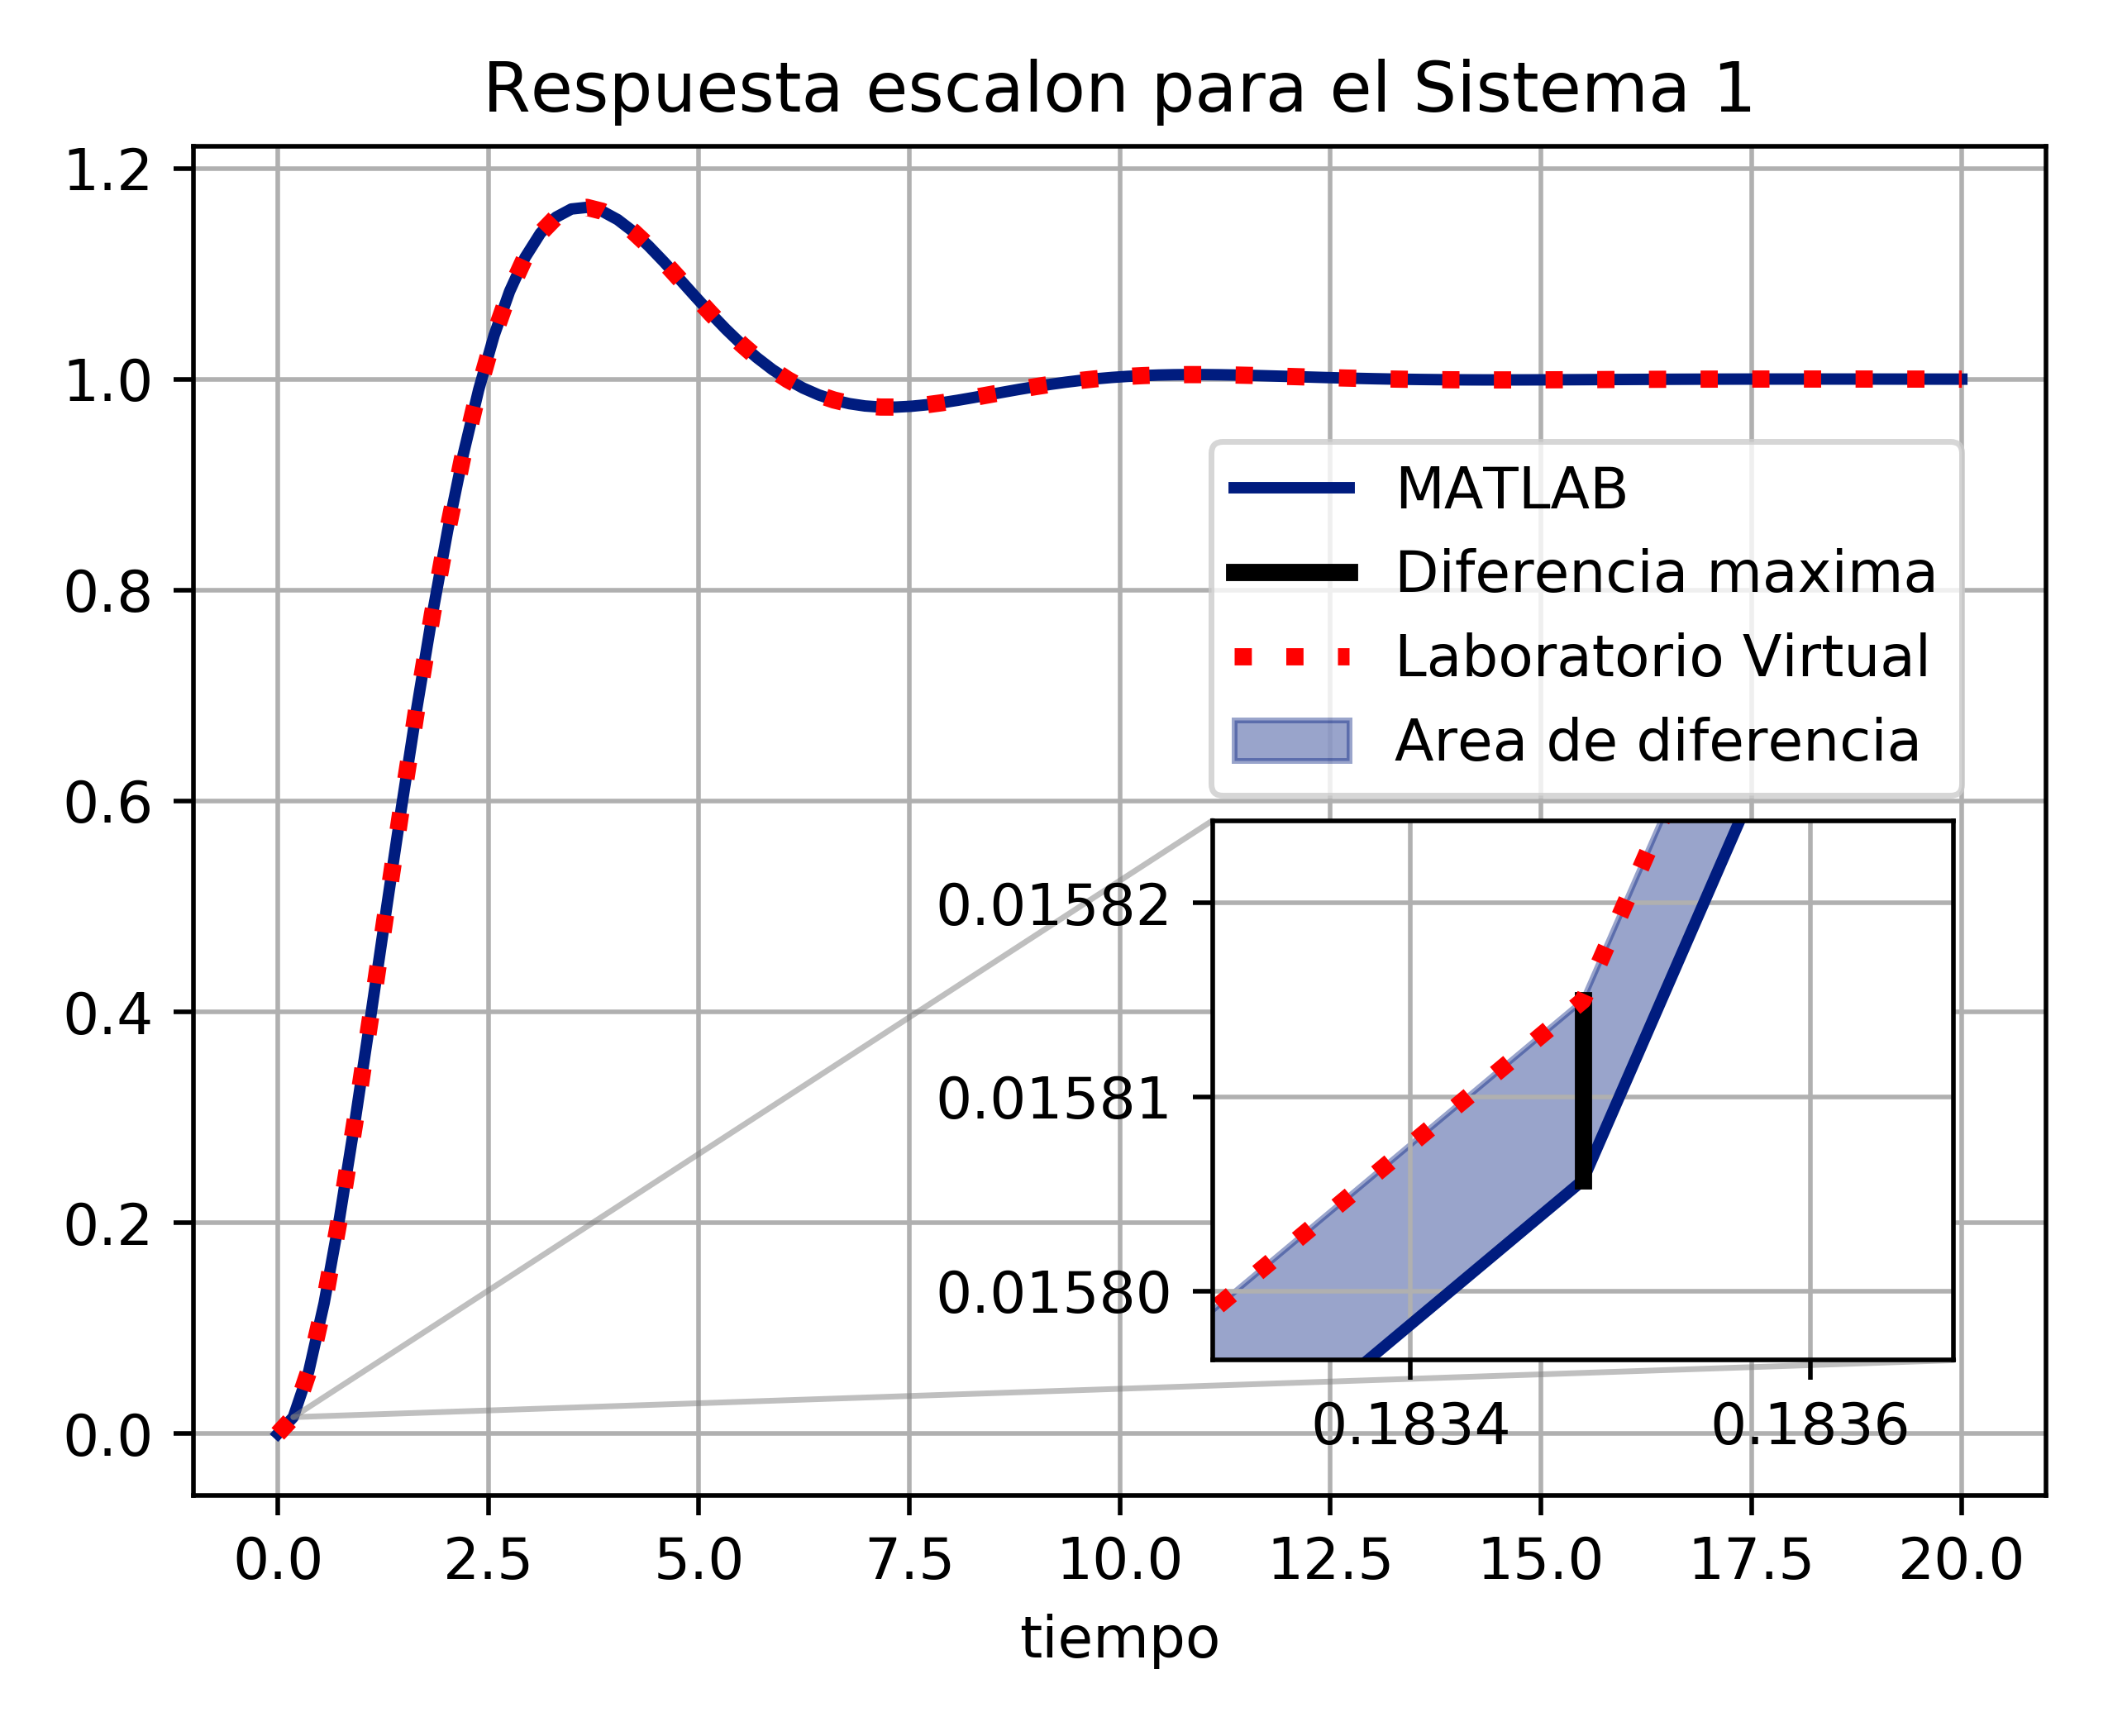
\includegraphics[width=0.49\textwidth,valign=c]{MATLAB/Set1Step.png}
                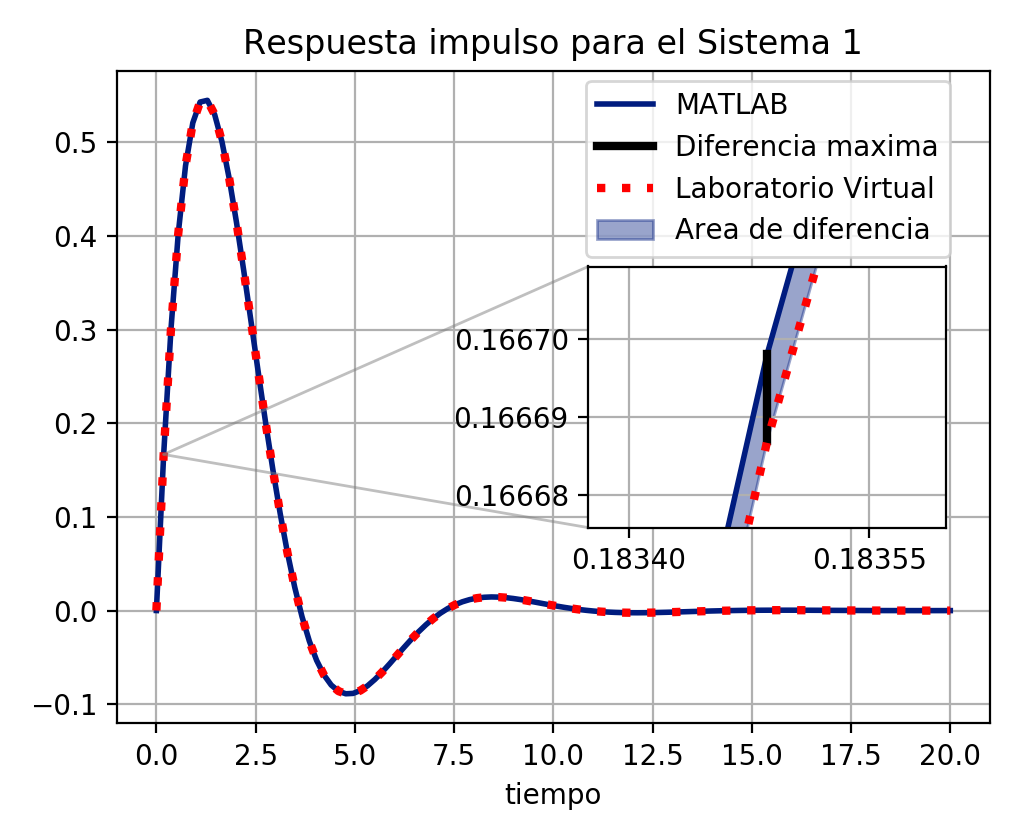
\includegraphics[width=0.49\textwidth,valign=c]{MATLAB/Set1Imp.png}
                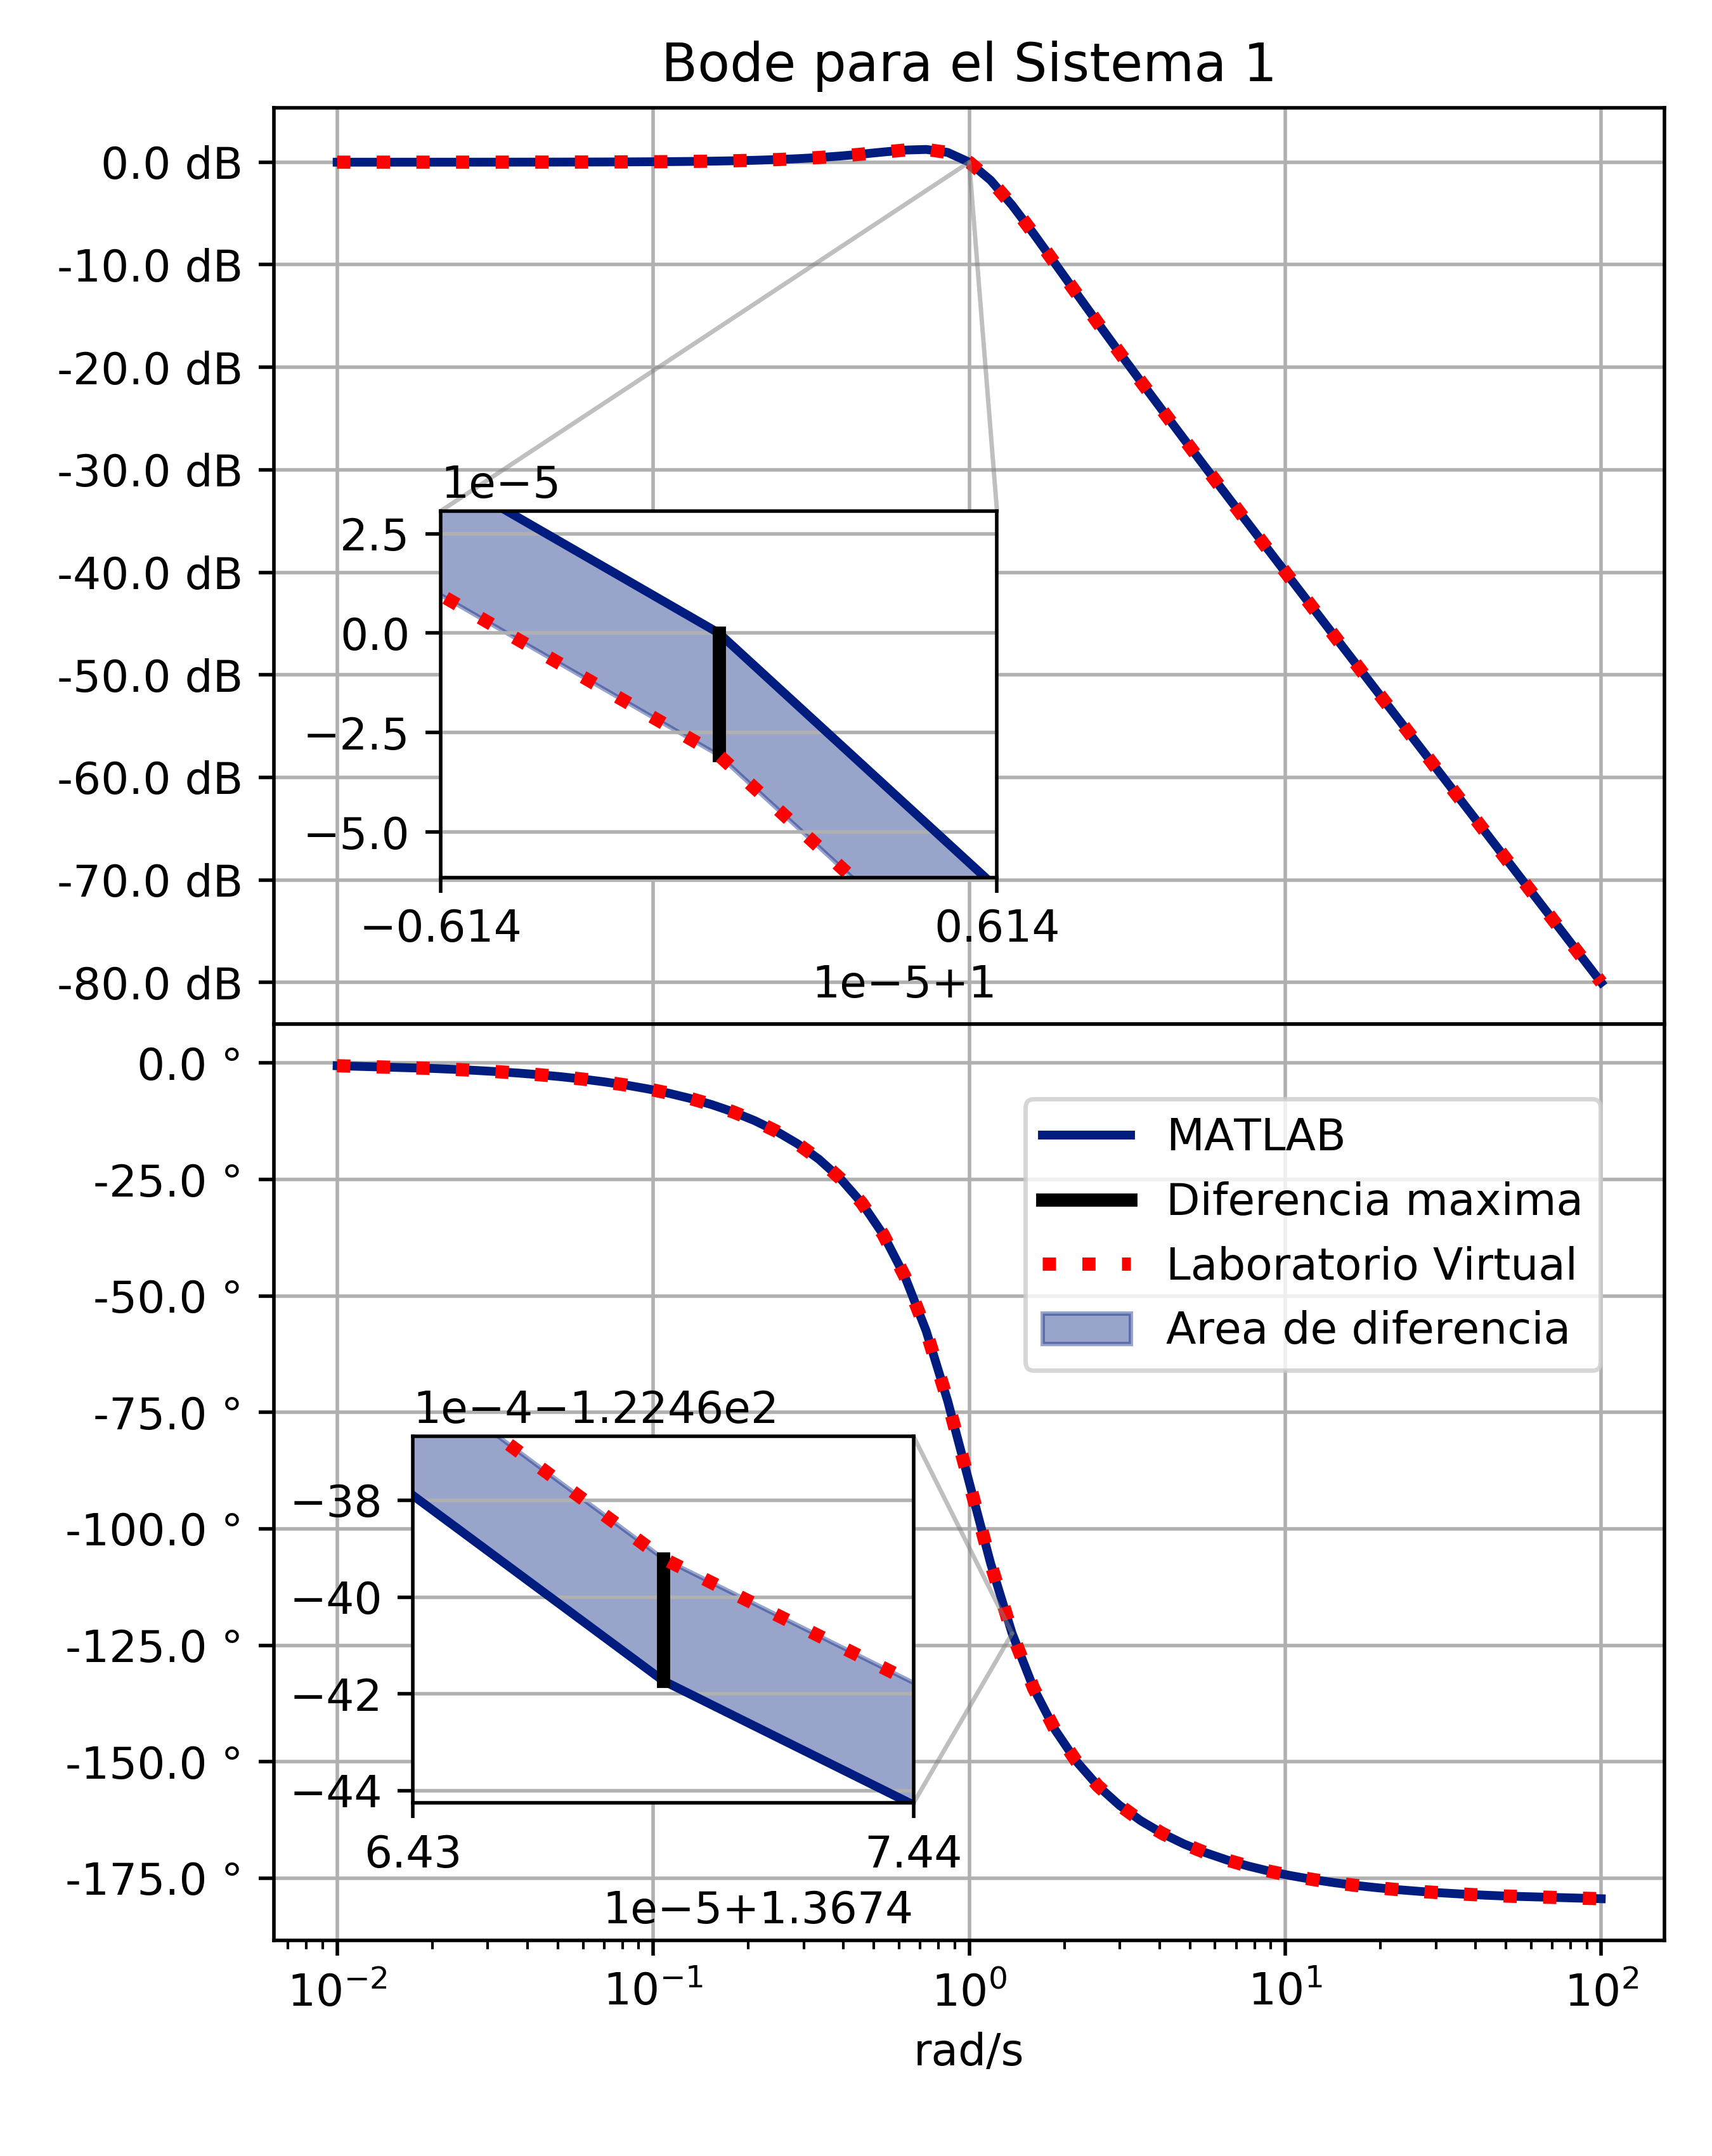
\includegraphics[width=0.49\textwidth,valign=c]{MATLAB/Set1Bode.png}
                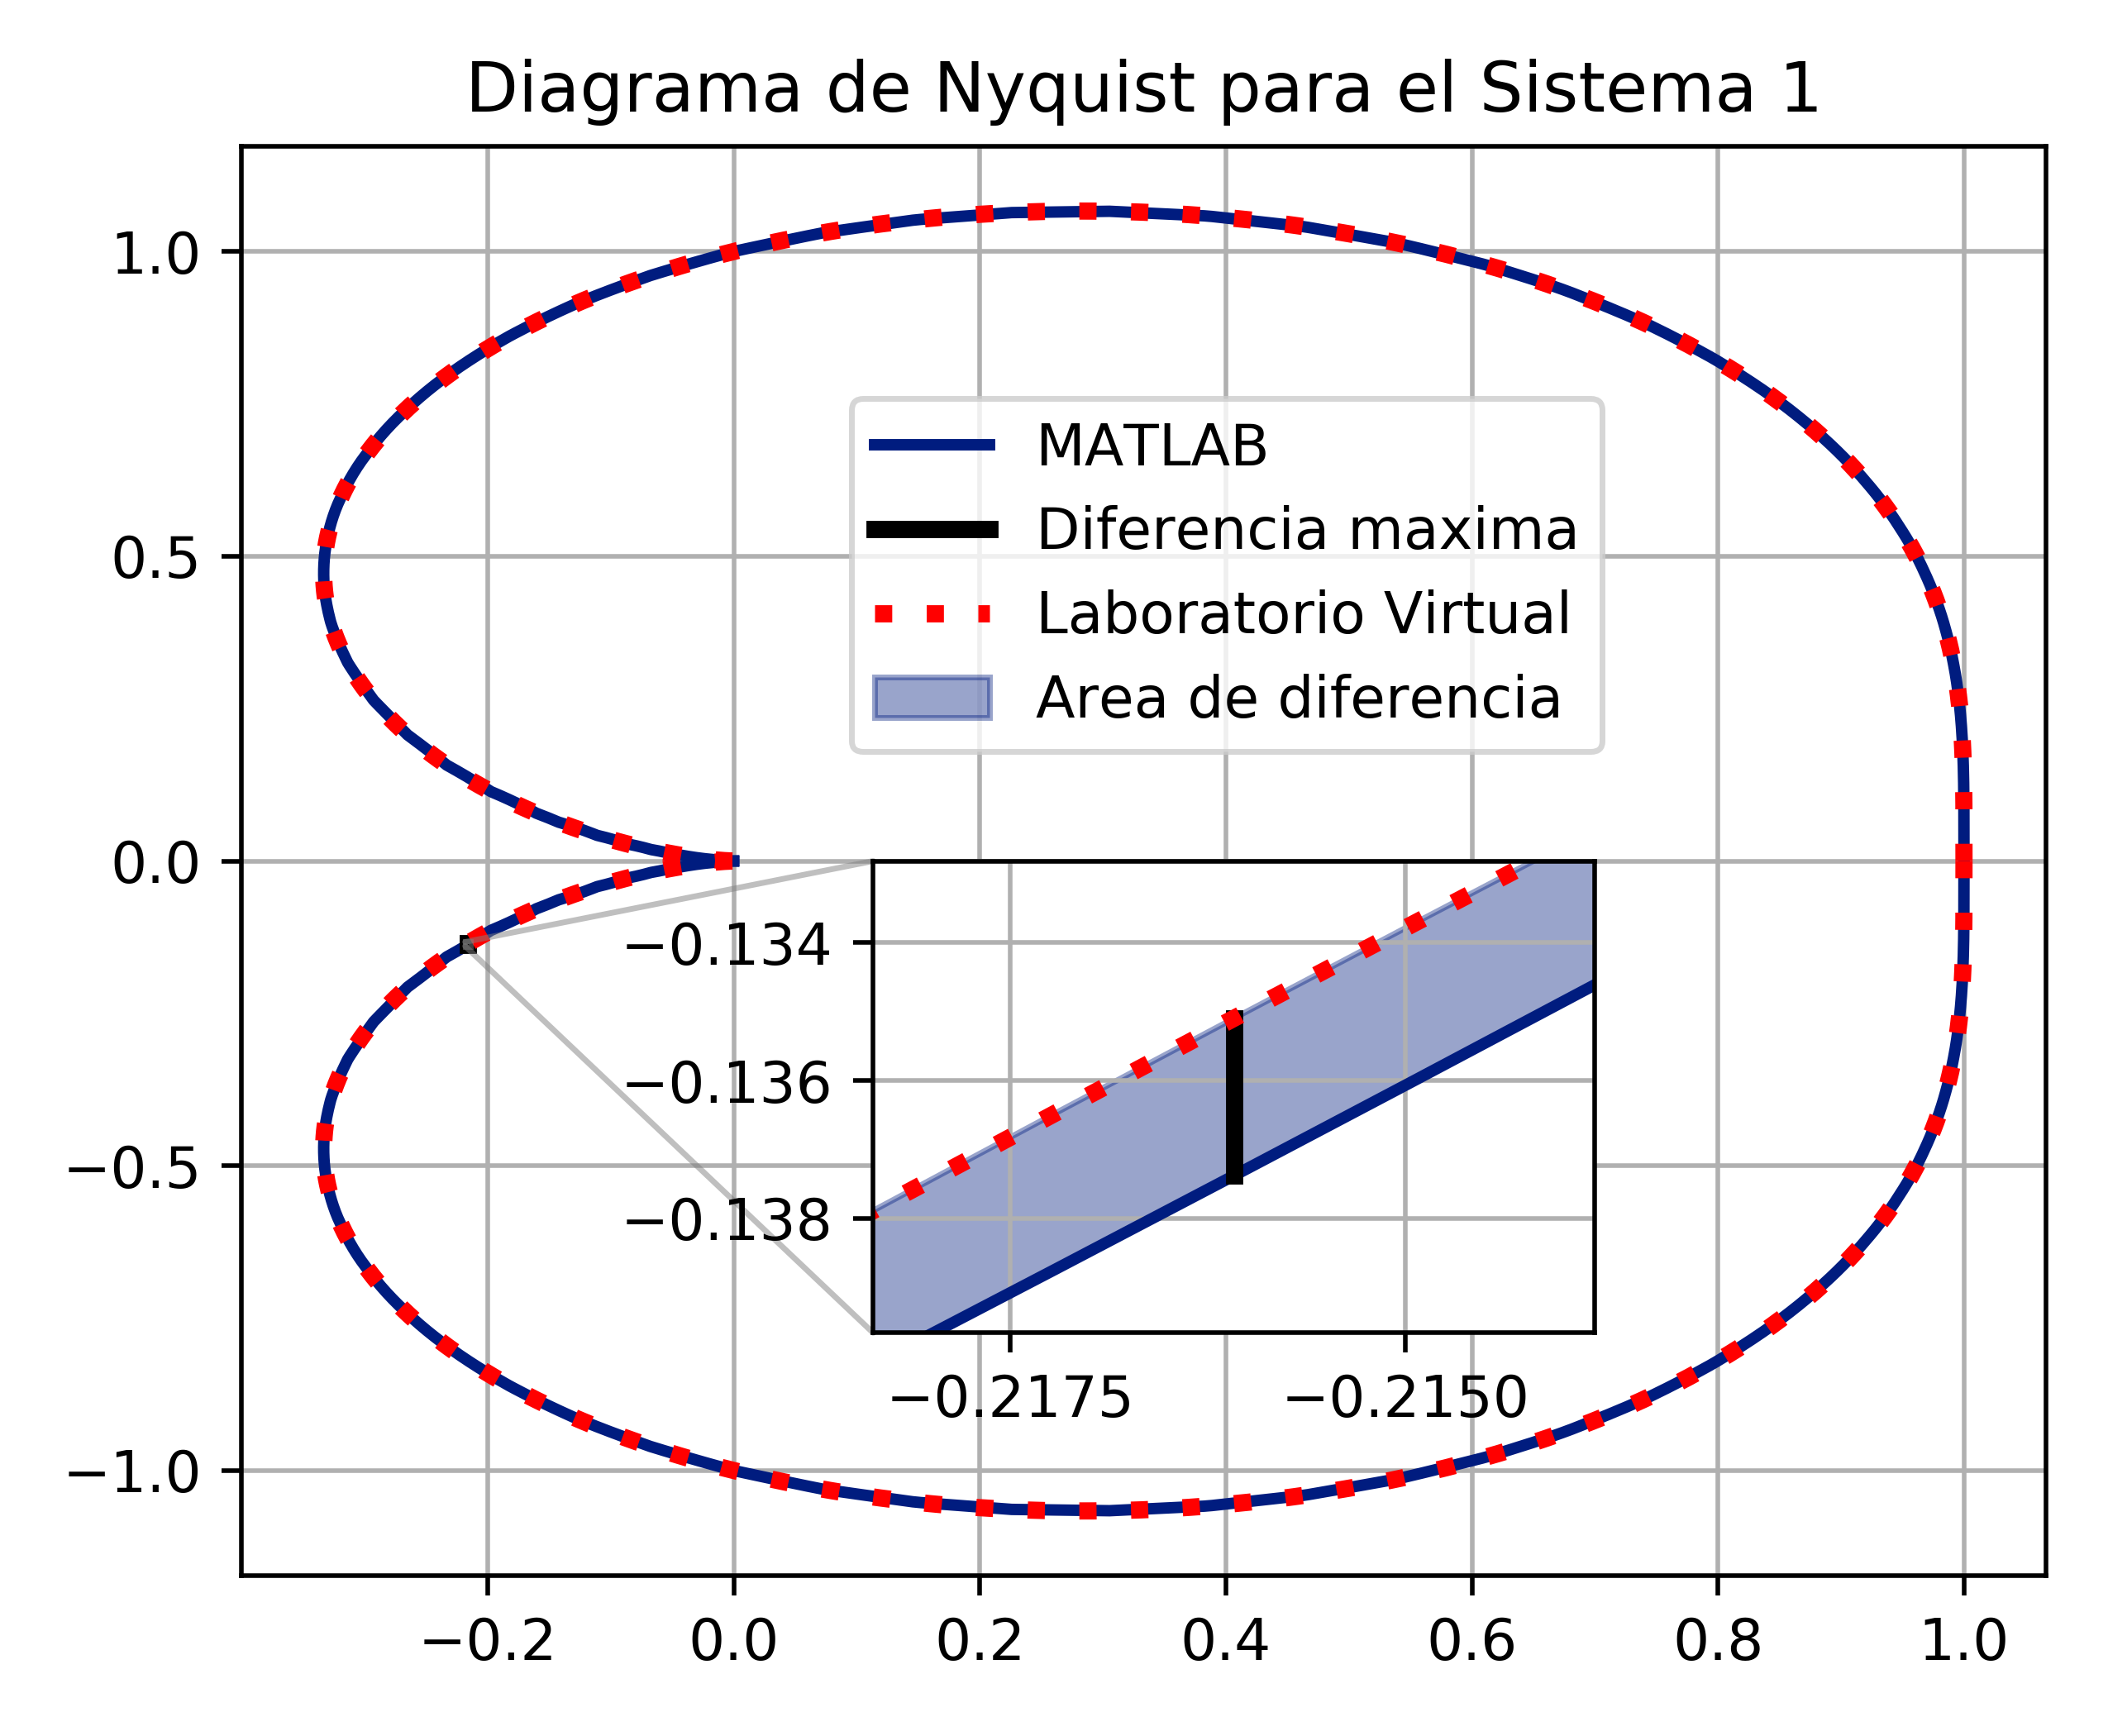
\includegraphics[width=0.49\textwidth,valign=c]{MATLAB/Set1Nyquist.png}
                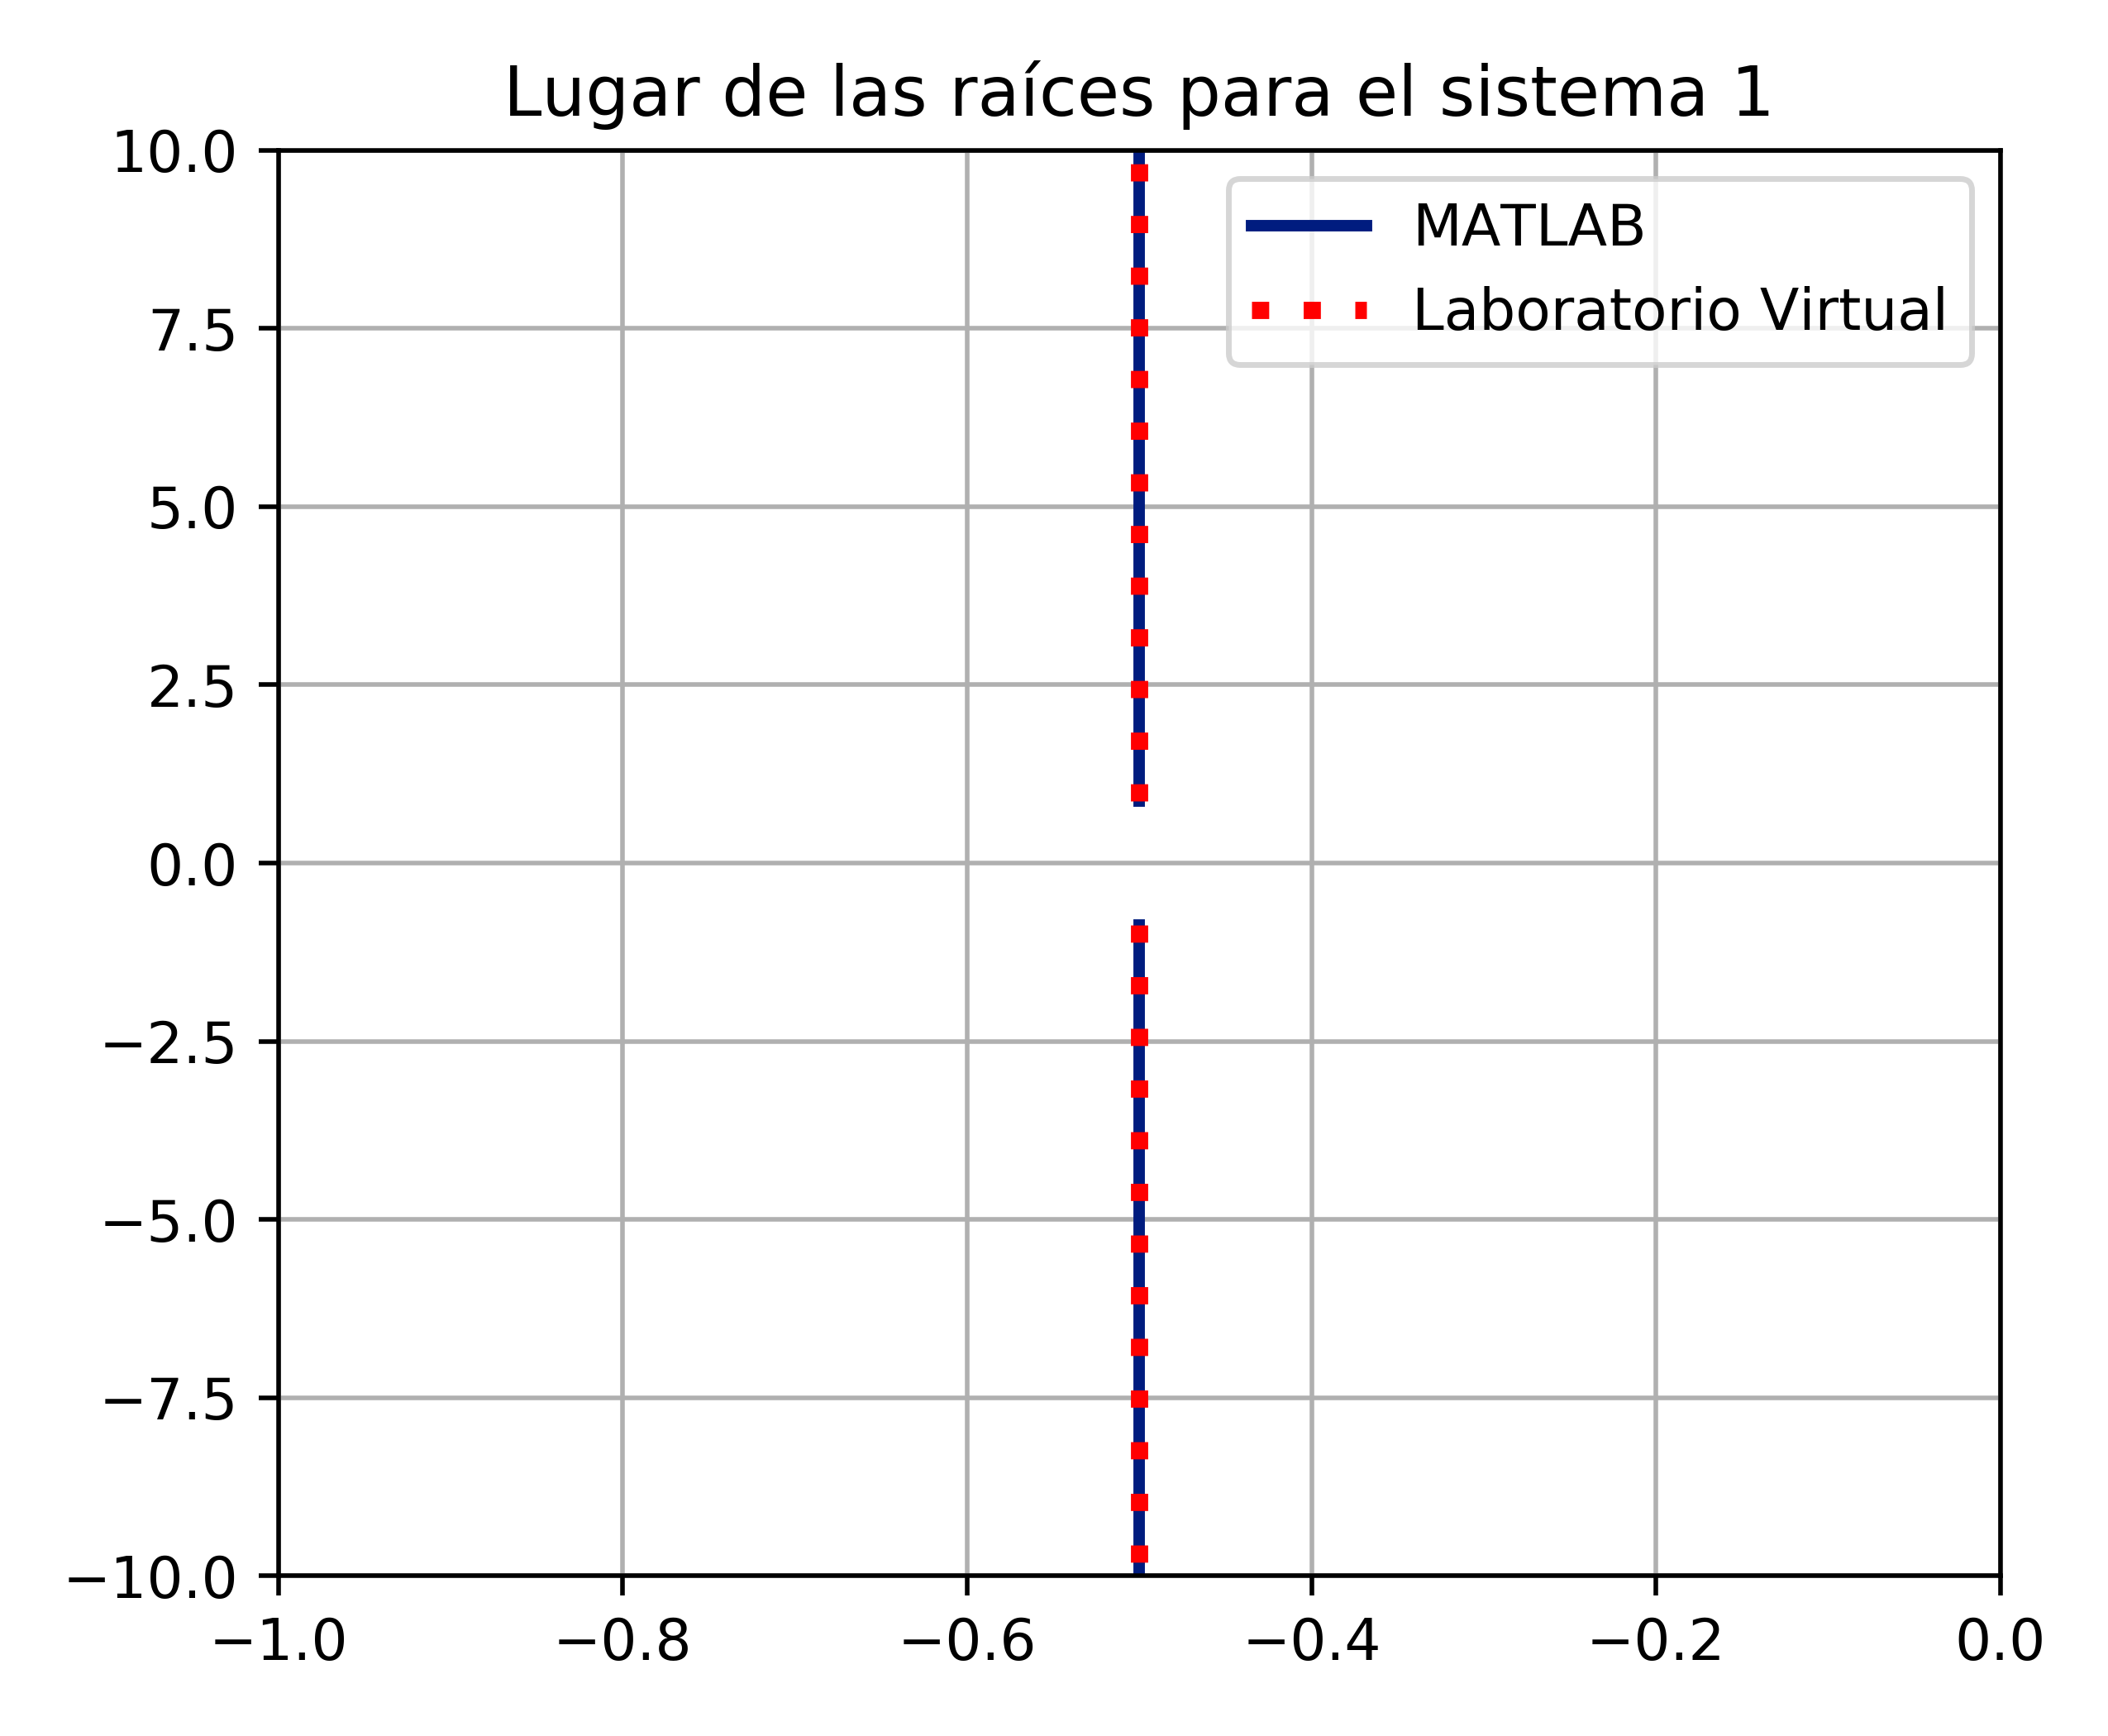
\includegraphics[width=0.49\textwidth,valign=c]{MATLAB/Set1Rlocus.png}
                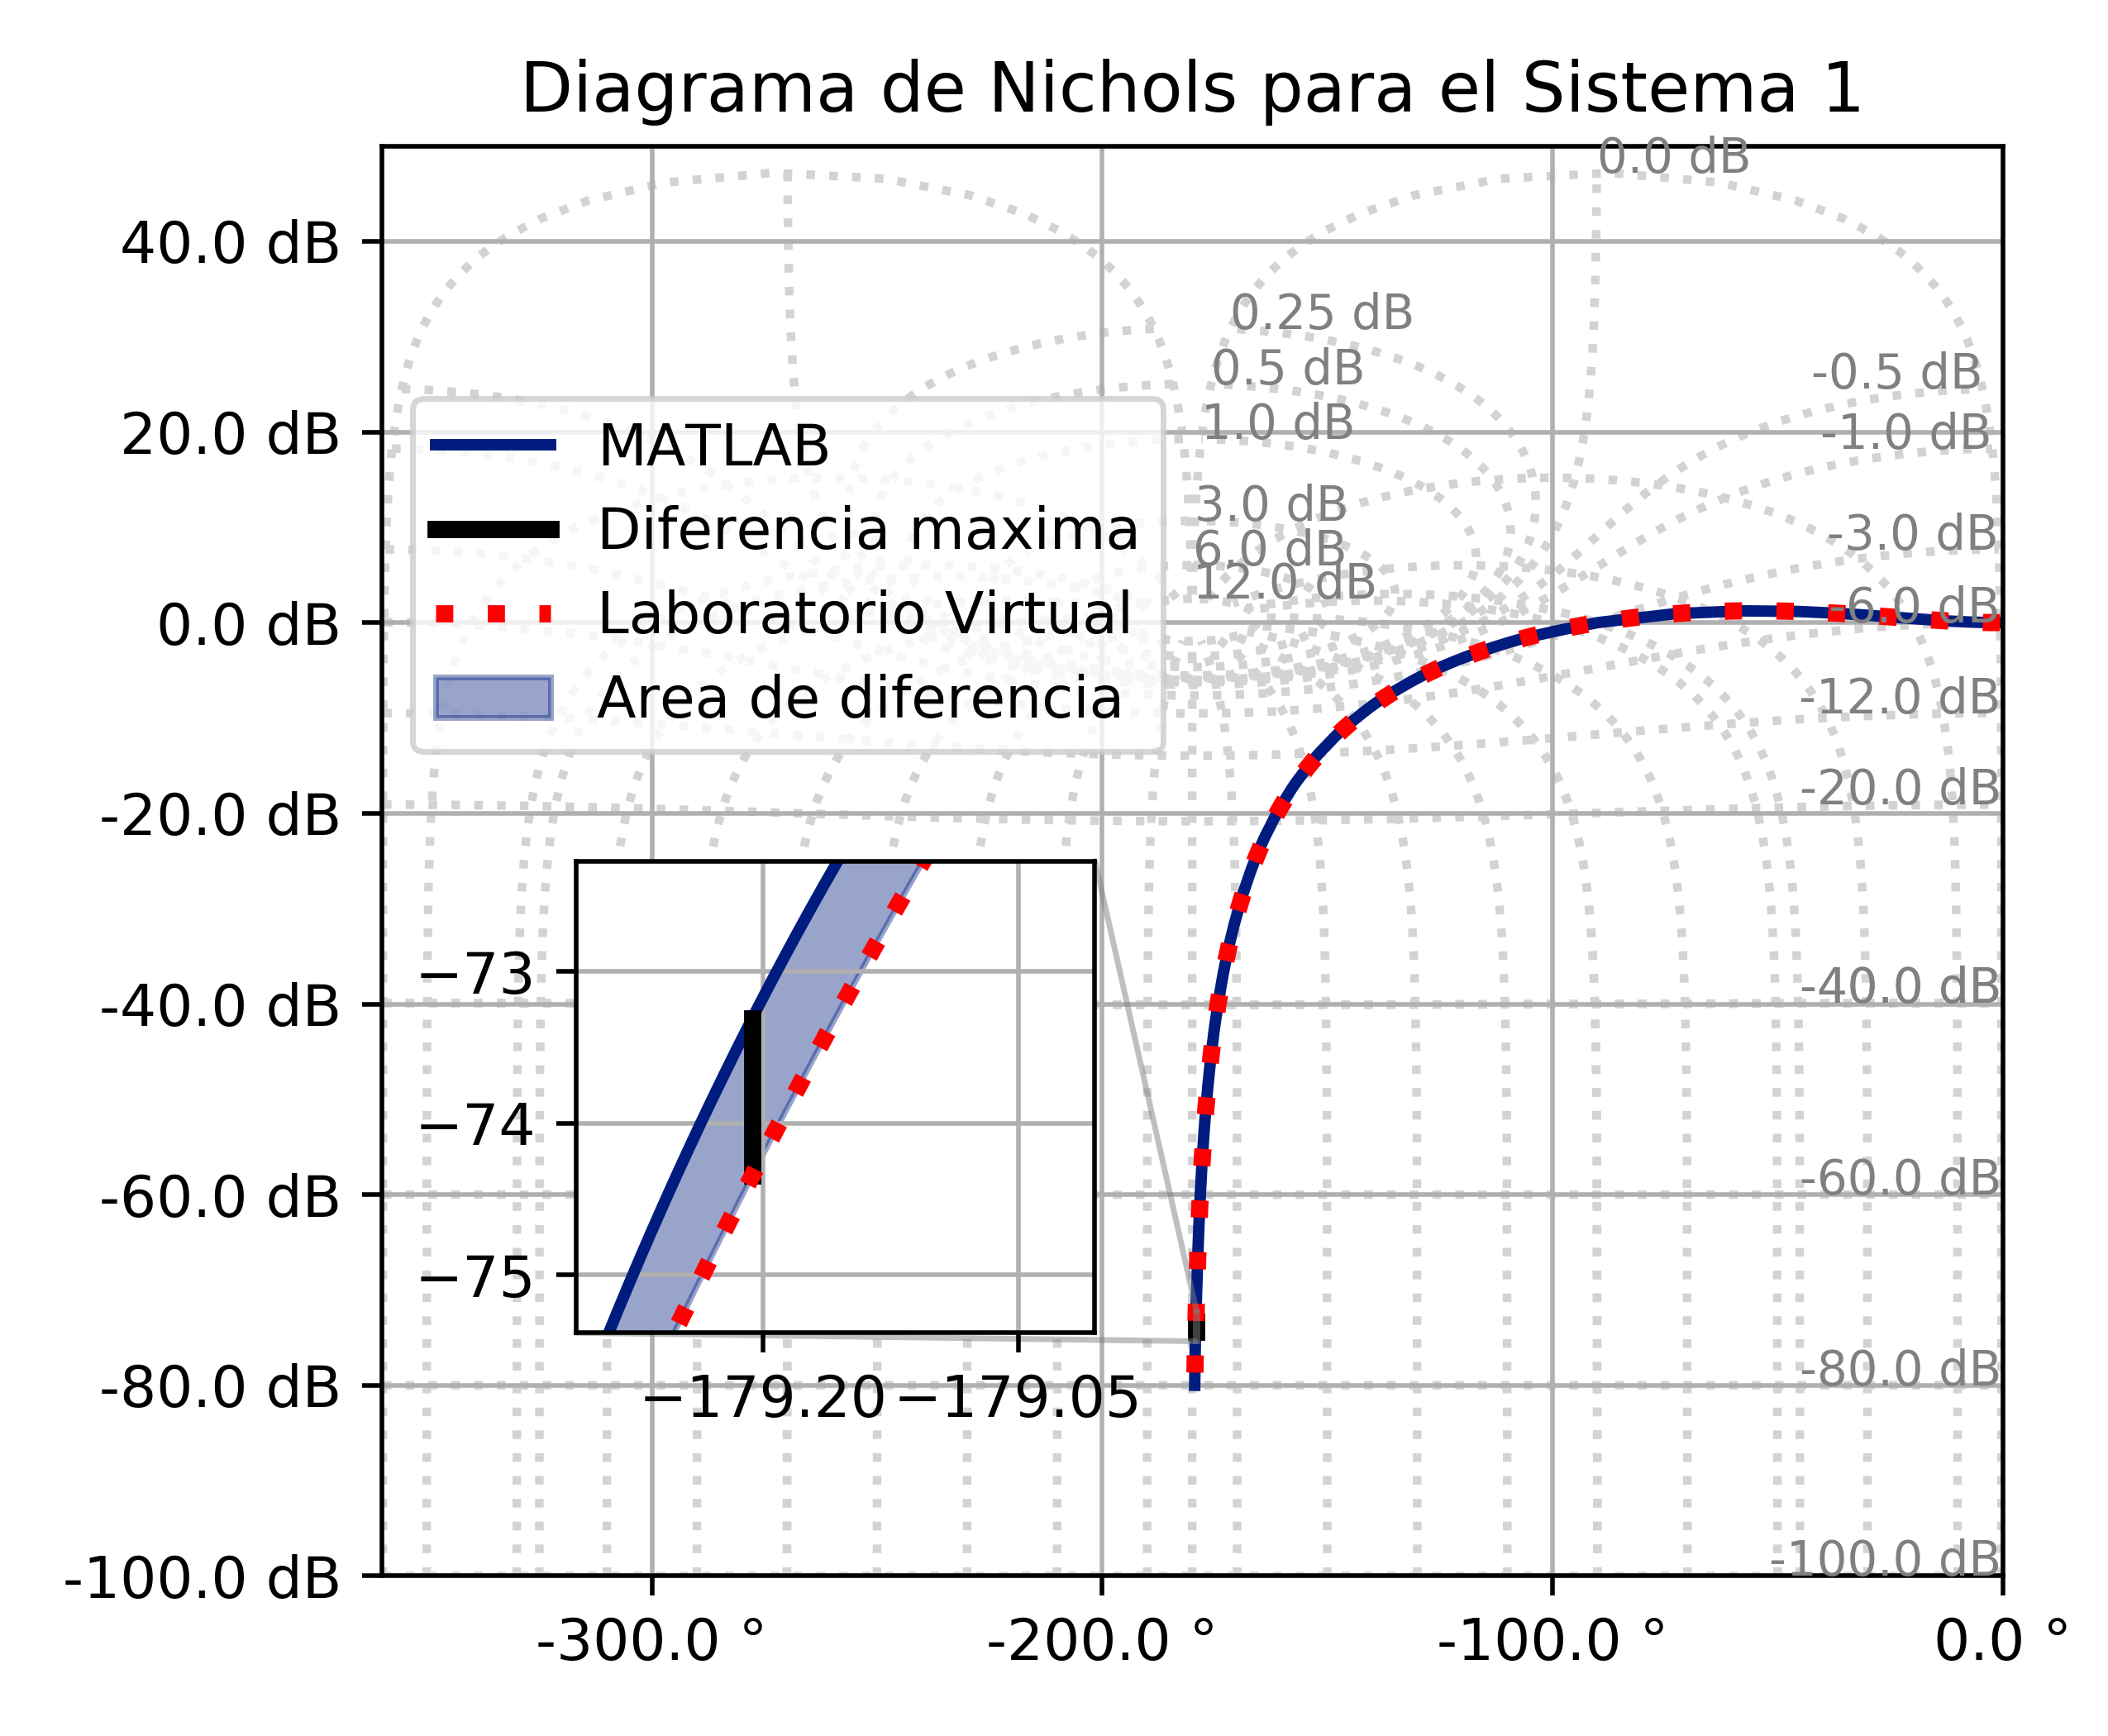
\includegraphics[width=0.49\textwidth,valign=c]{MATLAB/Set1Nichols.png}
                \label{fig:Set1sub}
            \end{subfigure}
            \caption[Comparacion de analisis/MATLAB - sistema continuo 1]{\textbf{Comparacion de analisis/MATLAB - sistema continuo 1}. Fuente: Elaboración propia. \label{fig:Set1}}
        \end{figure}

        \clearpage

        La anterior comparativa es basada en presicion utilizando las funciones de MATLAB y SciLab a base de codigo, no obstante, el Laboratorio Virtual permite realizar los analisis con solo definir el sistema a analizar, este metodo de analisis tambien se puede realizar en MATLAB con la aplicacion (app) Linear System Analyzer, la cual permite realizar las mismas funciones, en el caso de SciLab no existe una aplicacion similar.

    \subsection{Entonación de controladores PID}
        
        Para la funcion de entonacion de controladores PID no se realizo una comparacion numerica dado que los resultados seran los ya vistos en la funcion de analisis, por tanto, la comparacion se enfocara en la funcion per se y su forma de uso.

        El Laboratorio Virtual permite ajustar las ganancias del controlador PID con solo deslizar los sliders correspondientes, permitiendo visualizar los efectos del aumento de cada una de los componentes del controlador PID, a su vez, permite habilitar y deshabilitar cada componente de forma sencilla permitiendo asi, una forma visual de entonacion rapida y sin complicaciones. En el caso de MATLAB, existen varias herramientas de entonacion, la que presenta mayor similitud es el PID Tuner, el cual permite entonar el controlador basado en el tiempo de respuesta y en el transitorio, no permite ajustar de forma individual cada ganancia, pero si contiene otras funciones no disponibles en el Laboratorio Virtual. En el caso de SciLab, no existe ninguna herramienta que cumpla con la funcion de entonar controladores PID.

        En ambos casos, tanto el Laboratorio Virtual como el PID Tuner de MATLAB permite realizar una entonacion automatica y realizar ajustes finales de forma manual, el Laboratorio Virtual utiliza los metodos de Ziegler-Nichols y Cohen-Coon, en el caso de MATLAB no se conoce que metodo es utilizado. Para la identificacion y entonacion de sistemas a partir de data recolectada, MALTAB posee la aplicacion System Identification, la cual tiene una gran cantidad de opciones superiores al Laboratorio Virtual en lo que a identifiacion de sistemas respecta, no obstante, el Laboratorio Virtual tiene la ventaja de poseer una entonacion automatica al mismo tiempo que se realiza la identificacion. Nuevamente, SciLab no posee herramientas que puedan realizar identificacion de sistemas a partir de la data recolectada, si bien, las anteriores funciones pueden ser implementadas a codigo, el problema recae en el usuario.

    \subsection{Diseño de controladores difusos}

        
            